\chapter{Spinors: Spin 1/2 Fields}
\section{Dirac's Approach to RQM:}
Dirac's primary goal was a 1st order relativistic Schrodinger equation, and he postulated that if it existed, it must have the general form of 
\begin{equation}
i \frac{\partial}{\partial t}|\psi\rangle= H|\psi\rangle=(a \cdot \mathbf{p}+\beta m)|\psi\rangle
\label{1st-order-relativistic-SDE}
\end{equation}
In \ref{1st-order-relativistic-SDE}, $\mathbf{p}$ is particle three momentum (an operator in quantum theories), and the vector $\alpha$ and the scalar $\beta$ would have to be determined. Thus, the equation would be first order in the time derivative. To find $\alpha$ and $\beta$, Dirac reasoned that $H^{2}$ and $|\psi\rangle$ must also satisfy the usual relativistic energy momentum relation (and therefore the Klein-Gordon equation)
$$
-\frac{\partial^{2}}{\partial t^{2}}|\psi\rangle= H^{2}|\psi\rangle=\left(\mathbf{p}^{2}+m^{2}\right)|\psi\rangle
$$
Thus
$$
-\frac{\partial^{2}}{\partial t^{2}}|\psi\rangle= H^{2}|\psi\rangle=\left(\alpha_{i} p_{i}+\beta m\right)\left(\alpha_{j} p_{j}+\beta m\right)|\psi\rangle
$$
$$
=\left(\alpha_{i}^{2} p_{i}^{2}+\underbrace{\left(\alpha_{i} \alpha_{j}+\alpha_{j} \alpha_{i}\right)}_{\text {must }=0}p_{i}p_{j}+\underbrace{\left(\alpha_{i} \beta+\beta \alpha_{i}\right)}_{\text {must }=0} p_{i} m+\beta^{2} m^{2}\right)|\psi\rangle
$$
Therefore, $\alpha_{i}^{2}=1$ and $\beta^{2}=1$. In summary, we have anti-commutators relationship:
\begin{qt}
    \begin{equation}
\begin{aligned}
&\left[\alpha_{i}, \alpha_{j}\right]_{+}=\left[\alpha_{i}, \beta\right]_{+}=0 \quad i \neq j \quad \alpha_{1}, \alpha_{2}, \alpha_{3}, \beta \text { all anti-commute with each other, }\\
&\left(\alpha_{1}\right)^{2}=\left(\alpha_{2}\right)^{2}=\left(\alpha_{3}\right)^{2}=(\beta)^{2}=1 \text { (the identity matrix) }
\end{aligned}
\label{standard-condition}
\end{equation}
\end{qt}
\bluep{If $\alpha_{i}$ and $\beta$ were numbers they would have to commute and could not possibly anti-commute. Hence, they can only be matrices. since these matrices are operators operating on $|\psi\rangle,$ then $|\psi\rangle$ itself must be a multicomponent object (i.e., a column matrix, at least.)}. Use the relations above, one can show that the \redp{$\alpha$ and $\beta$ matrices are traceless, hermitian, have $\pm$ eigenvalues, and must have an even dimension of at least four}.

Square matrices in a 4D space must be  $4\mathrm{X} 4,$ and thus if $|\psi\rangle$ is a column matrix (a vector), it must have four components (a 4D vector). Take care to note the \bluep{4D space we are talking about here is not the four-dimensional physical space of relativity theory, but an abstract pace, often called \textbf{spinor space}}.
\subsection{Standard presentation}
Choosing the minimum dimension case (four), Dirac and Pauli came up with a set of matrices which solve all of the conditions in (\ref{standard-condition}):
$$
\beta=\left[\begin{array}{cccc}
{1} \\
{} & {1} \\
{} & {} & {-1} \\
{} & {} & {} & {-1}
\end{array}\right]
$$
$$
\alpha_{1}=\left[\begin{array}{cccc}
{}&{}&{}&{1} \\
{}&{}&{1} \\
{} & {1} \\
{1}
\end{array}\right] \quad \alpha_{2}=\left[\begin{array}{cccc}
{}&{}&{}&{-i} \\
{}&{}&{i} \\
{} & {-i} \\
{i}
\end{array}\right] \quad \alpha_{3}=\left[\begin{array}{cccc}
{}&{}&{1} \\
{}&{}&{}& {-1} \\
{1}\\
{}&{-1} 
\end{array}\right]
$$
which are commonly written using Pauli matrices
$$
\beta=\left[\begin{array}{cc}
{I} & {0} \\
{0} & {-I}
\end{array}\right] \quad \alpha_{1}=\left[\begin{array}{cc}
{0} & {\sigma_{1}} \\
{\sigma_{1}} & {0}
\end{array}\right] \quad \alpha_{2}=\left[\begin{array}{cc}
{0} & {\sigma_{2}} \\
{\sigma_{2}} & {0}
\end{array}\right] \quad \alpha_{3}=\left[\begin{array}{cc}
{0} & {\sigma_{3}} \\
{\sigma_{3}} & {0}
\end{array}\right]
$$
If we define \textbf{gamma matrices} or \redp{\textbf{Dirac matrices}} as:
\begin{equation}
\gamma^{0}=\beta \quad \gamma^{1}=\beta \alpha_{1} \quad \gamma^{2}=\beta \alpha_{2} \quad \gamma^{3}=\beta \alpha_{3}
\end{equation}
we find the \textbf{Hermiticity conditions} as
\begin{equation}
\gamma^{\mu \dagger}=\gamma^{0} \gamma^{\mu} \gamma^{0}
\end{equation}
\subsection{Dirac equation expressed with Dirac matrices}
Pre-multiplied $\beta$, Dirac's original $1^{st}$ order equation takes on the form
\begin{equation}
i \beta \frac{\partial}{\partial t}|\psi\rangle=\left(\beta \alpha_{i} p_{i}+\beta^{2} m\right) | \psi\rangle=\left(-i \gamma^{i} \frac{\partial}{\partial x^{i}}+m\right)|\psi\rangle
\end{equation}
or rearranged as what is formally called the \textbf{Dirac equation}:
\begin{equation}
\sum_{\eta=1}^{4}\left(\sum_{\mu=0}^{3} i\left(\gamma^{\mu}\right)_{\kappa \eta} \partial_{\mu}-m \delta_{\kappa \eta}\right)|\psi\rangle_{\eta}=0 \quad \kappa=1,2,3,4
\end{equation}
where we have written out the $4 \mathrm{X} 4$ spinor space indices in $\kappa$ and $\eta$. Note the Dirac equation is actually \textbf{four separate non-matrix equations}, one for each value of the index $\kappa$. And each of these equations entails a sum of matrix components (sum over $\mu$ ), each post multiplied by one of the four components (in $\eta$ index) of the column vector $|\psi\rangle$.
\begin{qt}
    The common way to write the Dirac equation is to hide the spinor space indices in $\kappa$ and $\eta$,
    \begin{equation}
\left(i \gamma^{\mu} \partial_{\mu}-m\right)|\psi\rangle= 0
\label{convenient-Dirac-eq}
\end{equation}
Another notation commonly used, which is the most streamlined of all, is
$$
\not \partial=\gamma^{\mu} \partial_{\mu} \quad \text { so, the Dirac equation } \rightarrow(i \not \partial-m)|\psi\rangle= 0
$$
\end{qt}
Also, $m \rightarrow \frac{m c}{\hbar} \quad$ in non-natural units in the Dirac equation.

\subsection{Solutions to the Dirac equation}
Write out (\ref{convenient-Dirac-eq}) fully as:
$$
i \gamma^{\mu} \partial_{\mu}|\psi\rangle= i\left(\gamma^{0} \partial_{0}+\gamma^{1} \partial_{1}+\gamma^{2} \partial_{2}+\gamma^{3} \partial_{3}\right)|\psi\rangle= m|\psi\rangle=
$$
$$
=i\left(\left[\begin{array}{cccc}
{\partial_{0}} & {0} & {\partial_{3}} & {\partial_{1}-i \partial_{2}} \\
{0} & {\partial_{0}} & {\partial_{1}+i \partial_{2}} & {-\partial_{3}} \\
{-\partial_{3}} & {-\partial_{1}+i \partial_{2}} & {-\partial_{0}} & {0} \\
{-\partial_{1}-i \partial_{2}} & {\partial_{3}} & {0} & {-\partial_{0}}
\end{array}\right]\right) \left| \begin{array}{l}
{\psi_{1}} \\
{\psi_{2}} \\
{\psi_{3}} \\
{\psi_{4}}
\end{array}\right\rangle=
m\left|\begin{array}{l}
{\psi_{1}} \\
{\psi_{2}} \\
{\psi_{3}} \\
{\psi_{4}}
\end{array}\right\rangle
$$
The Dirac equation solutions in the Dirac-Pauli (standard) representation are
\begin{qt}
$$
\left|\psi^{(1)}\right\rangle=\underbrace{\sqrt{\frac{E+m}{2 m}}\left(\begin{array}{c}
{1} \\
{0} \\
{\frac{p^{3}}{E+m}} \\
{\frac{p^{1}+i p^{2}}{E+m}}
\end{array}\right) }_{u_1} \underbrace{e^{-i p x}}_{\text {4D physical space part}}=u_1e^{-i p x}
$$
$$
\left|\psi^{(2)}\right\rangle=\underbrace{\sqrt{\frac{E+m}{2 m}}\left(\begin{array}{c}
{0} \\
{1} \\
{\frac{p^{1}-i p^{2}}{E+m}} \\
{\frac{-p^{3}}{E+m}}
\end{array}\right)}_{u_2} e^{-i p x}=u_2e^{-i p x}
$$
$$
\left|\psi^{(3)}\right\rangle=\underbrace{\sqrt{\frac{E+m}{2 m}}\left(\begin{array}{c}
{\frac{p^{3}}{E+m}} \\
{\frac{p^{1}+i p^{2}}{E+m}}\\
{1} \\
{0} 
\end{array}\right)}_{v_2} e^{i p x}=v_2e^{i p x}
$$
\begin{equation}
\left|\psi^{(4)}\right\rangle=\sqrt{\frac{E+m}{2 m}}\left(\begin{array}{c}
{\frac{p^{1}-i p^{2}}{E+m}}\\
{\frac{-p^{3}}{E+m}} \\
{0} \\
{1} 
\end{array}\right) e^{i p x}=v_1e^{i p x}
\label{four-spinors}
\end{equation}
\end{qt}
We have defined new symbols $u_{r}(\mathbf{p})$ and $v_{r}(\mathbf{p})(r=1,2),$ which are the column vectors multiplied by the constant shown, are functions only of $\mathbf{p}$ for a given $m(\text { since } E=\sqrt{\mathbf{p}^{2}+m^{2}}),$ and go by the name \textbf{spinors}, or \textbf{\redp{four-spinors}}. Note that \bluep{the particles represented by $|\psi^{(n)}\rangle$ are also often called spinors.}

\textbf{$u_{1}$ represents spin up, and $u_{2}$ represents spin down in the particle at-rest system. As you might expect, we will find the solutions containing $v_{r}(\mathbf{p})$ are associated with antiparticles; and those with $u_{r}(\mathbf{p}),$ with particles.}\redp{Take care to note the reverse order numbering on $v_{2,1}$ from $u_{1,2},$ which is customary.}

If we take \textbf{inner products of four spinors}, we have
$$
u_{1}^{\dagger}(\mathbf{p}) u_{1}(\mathbf{p})=\frac{E}{m}
$$
More generally
\begin{equation}
u_{\underline{r}L}^{\dagger}(\mathbf{p}) u_{\underline{r}}(\mathbf{p})=v_{\underline{r}}^{\dagger}(\mathbf{p}) v_{\underline{r}}(\mathbf{p})=\frac{E}{m}
\end{equation}
Where underline means no summation. Also, spinors are \textbf{orthogonal}
\begin{qt}
\begin{equation}
\begin{aligned}
&u_{r}^{\dagger}(\mathbf{p}) u_{s}(\mathbf{p})=v_{r}^{\dagger}(\mathbf{p}) v_{s}(\mathbf{p})=\frac{E}{m} \delta_{r s}\\
&u_{r}^{\dagger}(\mathbf{p}) v_{s}(-\mathbf{p})=0
\end{aligned}
\label{coefficient-orthogonality}
\end{equation}
\end{qt}
Therefore, the eigensolutions are also orthogonal
\begin{equation}
\left\langle\psi^{(m)} | \psi^{(n)}\right\rangle= 0 \text { for } m \neq n
\end{equation}
For example
$$
\left\langle\psi^{(1)} | \psi^{(3)}\right\rangle=\int u_{1}^{\dagger}(\mathbf{p}) e^{+i p x} v_{2}(\mathbf{p}) e^{+i p x} d^{3} x=\underbrace{u_{1}^{\dagger}(\mathbf{p}) v_{2}(\mathbf{p})}_{=0 \text { for } \mathbf{p}=0} \underbrace{\int e^{+i p x} e^{+i p x} d^{3} x}_{=0 \text { for } \mathbf{p} \neq 0}=0
$$
where we follow \textbf{Cesaro integration}:$\int_{0}^{\infty} \sin x d x=1$ and $\int_{0}^{\infty} \cos x d x=0$.
\begin{qt}
The most general solution to the Dirac equation is:
\begin{equation}
\psi_{\text {state}}=|\psi\rangle=\sum_{r, \mathbf{p}} \sqrt{\frac{m}{V E_{\mathrm{p}}}}\left(C_{r}(\mathbf{p}) u_{r}(\mathbf{p}) e^{-i p x}+D_{r}^{\dagger}(\mathbf{p}) v_{r}(\mathbf{p}) e^{i p x}\right)
\label{general-Dirac-state}
\end{equation}
Unlike the Klein-Gordon equation, the Dirac equation is a matrix equation. So, rather than complex conjugate form of the wave equation, we need to consider \textbf{taking a complex conjugate pose of that equation}, we define  and use the \textbf{adjoint}
\begin{equation}
\bar{\psi}_{\text {state}}=\psi_{\text {state}}^{\dagger} \gamma^{0}=|\psi\rangle^{\dagger} \gamma^{0}=\left\langle\psi\left|\gamma^{0}=\langle\bar{\psi}|\right.\right.
\end{equation}
\redp{where an inner product between the row vector $|\psi\rangle^{\dagger}=\langle\psi|=\psi^{+}$ state and the gamma matrix are implied.} The adjoint Dirac equation is
\begin{equation}
i \partial_{\mu}\left\langle\bar{\psi}\left|\gamma^{\mu}+m\langle\bar{\psi}|=0\right.\right.
\label{adjoint-Dirac-eq}
\end{equation}
\end{qt}
Adjoint spinors are defined as the row vectors
\begin{equation}
\bar{u}_{r}=u_{r}^{\dagger} \gamma^{0} \quad \bar{v}_{r}=v_{r}^{\dagger} \gamma^{0}
\end{equation}
which, gives us the \textbf{\underline{discrete plane wave adjoint general solution form}}:
\begin{equation}
\bar{\psi}_{\text {state}}=\langle\bar{\psi}|=\sum_{r, \mathrm{p}} \sqrt{\frac{m}{V E_{\mathrm{p}}}}\left(D_{r}(\mathrm{p}) \bar{v}_{\mathrm{r}}(\mathrm{p}) e^{-i p x}+C_{r}^{\dagger}(\mathrm{p}) \bar{u}_{r}(\mathrm{p}) e^{i p x}\right)
\end{equation}
\subsection{Probability density for Dirac Fermions}
The \textbf{four-current} using the Dirac equation can be found to be
\begin{qt}
\begin{equation}
\partial_{\mu} j^{\mu}=0 \quad j^{\mu}=(\rho, \mathbf{j})=\bar{\psi}_{\text {state }} \gamma^{\mu} \psi_{\text {state }}=\left\langle\bar{\psi}\left|\gamma^{\mu}\right| \psi\right\rangle_{\text {not integ }}
\label{four-current-Dirac}
\end{equation}
where the subscript "not intg" means we are not integrating over space in the bracket shown.
\end{qt}
The (\ref{four-current-Dirac}) means the total quantity
\begin{equation}
\begin{aligned}
\int_{V} j^{0} d^{3} x &=\int_{V} \rho d^{3} x=\int_{V} \bar{\psi}_{\text {state}} \gamma^{0} \psi_{\text {state}} d^{3} x=\left\langle\bar{\psi}\left|\gamma^{0}\right| \psi\right\rangle \\
&=\int_{V} \psi_{\text {state}}^{\dagger} \gamma^{0} \gamma^{0} \psi_{\text {state}} d^{3} x=\langle\psi | \psi\rangle= Q^{\prime}
\end{aligned}
\end{equation}
is conserved for $V$= all space. \textbf{For a single particle state in RQM, if we assume the solution onlu terms with coefficients $C_r$}(i.e., only has spinors of form $u_r$), our $\rho$ becomes
\begin{equation}
\begin{aligned}
\rho &\left.=\left(\sum_{r, p} \sqrt{\frac{m}{V E_{p}}} C_{r}^{\dagger}(p) \underbrace{\bar{u}_{r}(p)}_{u_{r}^{\dagger}(p) \gamma^{o}}\right)e^{i p x}\right) \gamma^{0}\left(\sum_{r^{\prime}, p^{\prime}} \sqrt{\frac{m}{V E_{p^{p}}}} C_{r^{\prime}}\left(p^{\prime}\right) u_{r^{\prime}}^{\prime}\left(p^{\prime}\right) e^{-i p^{\prime} x}\right) \\
&=\left(\sum_{r, p} \sqrt{\frac{m}{V E_{p}}} C_{r}^{\dagger}(p) u_{r}^{\dagger}(p) e^{i p x}\right)\left(\sum_{r^{\prime}, p^{\prime}} \sqrt{\frac{m}{V E_{p}}} C_{r^{\prime}}\left(p^{\prime}\right) u_{r^{\prime}}\left(p^{\prime}\right) e^{-i p^{\prime} x}\right)
\end{aligned}
\end{equation}
If this is probability density, we have
$$
\int \rho d^{3} x=\sum_{r, p} \frac{m}{V}\left(C_{r}^{\dagger}(\mathrm{p}) C_{r}(\mathrm{p}) \frac{u_{r}^{\dagger}(\mathbf{p}) u_{r}(\mathrm{p})}{E_{p} / m} \underbrace{\int e^{-i p x}e^{ip x}d^{3} x}_{V}\right)==\sum_{r, \mathrm{p}}\left|C_{r}(\mathrm{p})\right|^{2}=1
$$
\bluep{Notice that a Dirac fermion represented by a solution with exponential form $-ipx$(that has spinor $u_r$ and coefficient $C_r(\mathbf{p})$), has positive energy; and one represented by solution form $ipx$(spinor $v_{r}$ and coefficient $D_{r}^{\dagger}(\mathrm{p})$ ), has negative energy.}

\subsection{Dirac approach to Spin}
\redp{The RQM spin operator} are defined as:
\begin{qt}
\begin{equation}
 \Sigma_{1}=\frac{\hbar}{2}\left[\begin{array}{cccc}
{} & {1} & {} & {} \\
{1} & {} & {} & {} \\
{} & {} & {} & {1} \\
{} & {} & {1} & {}
\end{array}\right] \Sigma_{2}=\frac{\hbar}{2}\left[\begin{array}{cccc}
{} & {-i} & {} & {} \\
{i} & {} & {} & {} \\
{} & {} & {} & {-i} \\
{} & {} & {i} & {}
\end{array}\right] \Sigma_{3}=\frac{\hbar}{2}\left[\begin{array}{cccc}
{1} & {} & {} & {} \\
{} & {-1} & {} & {} \\
{} & {} & {1} & {} \\
{} & {} & {} & {-1}
\end{array}\right]
\label{RQM-spin-operators}
\end{equation}
\end{qt}
Note $\Sigma_i$ (\ref{RQM-spin-operators}) is a $3 \mathrm{D}$ object in physical space (3 components of the spin angular momentum), but \textbf{each of the components in that space is itself a $4 \mathrm{X} 4$ matrix in relativistic $4 \mathrm{D}$ spinor space, rather than non-relativistic 2 D spinor space of NRQM.} \redp{In relativity. spin has three spatial components. But, relativistically, each component must act on a $4 \mathrm{D}$ column vector in spinor space.}

Consider a stationary Dirac particle which has $\mathrm{p}=0$ in our frame, and the solutions (\ref{four-spinors}) become much simplified. What then, are their respective spins? For the first such solution, we have
$$
\Sigma_{3}\left|\psi^{(1)}\right\rangle=\frac{\hbar}{2}\left[\begin{array}{cccc}
{1} \\
{}&{-1} \\
{} & {} & {1}\\
{} &{} &{}& {-1}
\end{array}\right] \sqrt{\frac{m+m}{2 m}}\left(\begin{array}{l}
{1} \\
{0} \\
{0} \\
{0}
\end{array}\right) e^{-i p x}=\frac{\hbar}{2}\left(\begin{array}{l}
{1} \\
{0} \\
{0} \\
{0}
\end{array}\right) e^{-i p x}=\frac{\hbar}{2}\left|\psi^{(1)}\right\rangle
$$
Therefore \textbf{\underline{$\left|\psi^{(1)}\right\rangle$ is for spin up.}}

As soon as we have a moving particle, things get more complicated, as we have to include nonzero $p^{i}$ values in our solutions (\ref{four-spinors}) This complication, which we didn't have in $\mathrm{NRQM},$ is due to relativistic effects.
\begin{mybox}
\textbf{Classical Macroscopic Spinning Object Translating at Relativistic Speed}

In $4 \mathrm{D}$ relativistic theory, angular momentum is a $2^{\mathrm{nd}}$ order tensor, but it can be treated simply as a vector formed from the integral over a rotating body of $d m\left(\mathbf{r} \times \mathbf{v}_{t}\right)=d m(\mathbf{r} \times(\omega \times \mathbf{r})),$ where symbols should be obvious. When a macroscopic object like a spinning disk, as shown below, moves close to the speed of light, distances contract in the direction of the velocity, and this makes the plane of the disk appear to turn. (See figure below.)
\end{mybox}
\begin{figure}[H]
    \centering
    \tikzset{every picture/.style={line width=0.75pt}} %set default line width to 0.75pt        
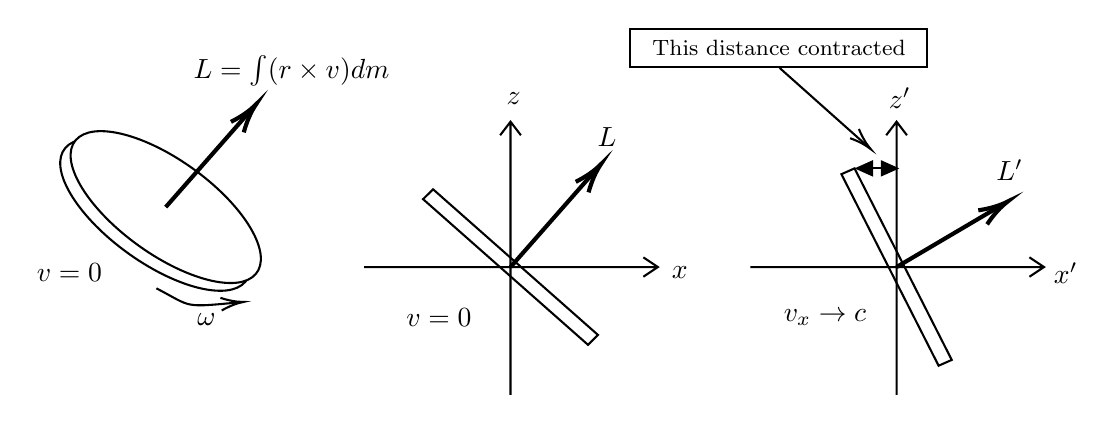
\begin{tikzpicture}[x=0.75pt,y=0.7pt,yscale=-1,xscale=1]
%uncomment if require: \path (0,300); %set diagram left start at 0, and has height of 300

%Shape: Ellipse [id:dp6696584947764774] 
\draw   (105.99,95.55) .. controls (114.14,85.31) and (140.18,92.46) .. (164.14,111.53) .. controls (188.1,130.6) and (200.92,154.36) .. (192.77,164.6) .. controls (184.62,174.85) and (158.58,167.7) .. (134.62,148.63) .. controls (110.66,129.56) and (97.84,105.8) .. (105.99,95.55) -- cycle ;
%Shape: Ellipse [id:dp8843951455763316] 
\draw  [fill={rgb, 255:red, 255; green, 255; blue, 255 }  ,fill opacity=1 ] (110.99,91.55) .. controls (119.14,81.31) and (145.18,88.46) .. (169.14,107.53) .. controls (193.1,126.6) and (205.92,150.36) .. (197.77,160.6) .. controls (189.62,170.85) and (163.58,163.7) .. (139.62,144.63) .. controls (115.66,125.56) and (102.84,101.8) .. (110.99,91.55) -- cycle ;
%Straight Lines [id:da6714691596952527] 
\draw [line width=1.5]    (154.38,126.08) -- (196,75.35) ;
\draw [shift={(197.9,73.03)}, rotate = 489.37] [color={rgb, 255:red, 0; green, 0; blue, 0 }  ][line width=1.5]    (14.21,-4.28) .. controls (9.04,-1.82) and (4.3,-0.39) .. (0,0) .. controls (4.3,0.39) and (9.04,1.82) .. (14.21,4.28)   ;

%Curve Lines [id:da608409716212424] 
\draw    (149.9,168.03) .. controls (167.54,177.83) and (162.13,178.03) .. (190.14,175.21) ;
\draw [shift={(191.9,175.03)}, rotate = 534.29] [color={rgb, 255:red, 0; green, 0; blue, 0 }  ][line width=0.75]    (10.93,-3.29) .. controls (6.95,-1.4) and (3.31,-0.3) .. (0,0) .. controls (3.31,0.3) and (6.95,1.4) .. (10.93,3.29)   ;

%Shape: Rectangle [id:dp2988248655701031] 
\draw  [fill={rgb, 255:red, 255; green, 255; blue, 255 }  ,fill opacity=1 ] (283.18,116.89) -- (362.64,192.09) -- (357.82,197.17) -- (278.36,121.98) -- cycle ;
%Shape: Axis 2D [id:dp3998228460871881] 
\draw [line width=0.75]  (250,157.03) -- (391.5,157.03)(320.5,82) -- (320.5,223.03) (384.5,152.03) -- (391.5,157.03) -- (384.5,162.03) (315.5,89) -- (320.5,82) -- (325.5,89)  ;
%Straight Lines [id:da08204495575914073] 
\draw [line width=1.5]    (320.5,157.03) -- (362.12,106.31) ;
\draw [shift={(364.02,103.99)}, rotate = 489.37] [color={rgb, 255:red, 0; green, 0; blue, 0 }  ][line width=1.5]    (14.21,-4.28) .. controls (9.04,-1.82) and (4.3,-0.39) .. (0,0) .. controls (4.3,0.39) and (9.04,1.82) .. (14.21,4.28)   ;

%Shape: Rectangle [id:dp9756203932975158] 
\draw  [fill={rgb, 255:red, 255; green, 255; blue, 255 }  ,fill opacity=1 ] (486.24,106.1) -- (533.08,204.97) -- (526.76,207.96) -- (479.92,109.1) -- cycle ;
%Shape: Axis 2D [id:dp2253494066411521] 
\draw [line width=0.75]  (436,157.03) -- (577.5,157.03)(506.5,82) -- (506.5,223.03) (570.5,152.03) -- (577.5,157.03) -- (570.5,162.03) (501.5,89) -- (506.5,82) -- (511.5,89)  ;
%Straight Lines [id:da26681235965231986] 
\draw [line width=1.5]    (506.5,157.03) -- (557.46,124.84) ;
\draw [shift={(560,123.23)}, rotate = 507.72] [color={rgb, 255:red, 0; green, 0; blue, 0 }  ][line width=1.5]    (14.21,-4.28) .. controls (9.04,-1.82) and (4.3,-0.39) .. (0,0) .. controls (4.3,0.39) and (9.04,1.82) .. (14.21,4.28)   ;

%Straight Lines [id:da2736459794596652] 
\draw    (489.24,106.1) -- (504.8,106.1) ;
\draw [shift={(507.8,106.1)}, rotate = 180] [fill={rgb, 255:red, 0; green, 0; blue, 0 }  ][line width=0.08]  [draw opacity=0] (8.93,-4.29) -- (0,0) -- (8.93,4.29) -- cycle    ;
\draw [shift={(486.24,106.1)}, rotate = 0] [fill={rgb, 255:red, 0; green, 0; blue, 0 }  ][line width=0.08]  [draw opacity=0] (8.93,-4.29) -- (0,0) -- (8.93,4.29) -- cycle    ;
%Straight Lines [id:da8576239603286319] 
\draw    (450.13,54.23) -- (492.69,94.85) ;
\draw [shift={(494.13,96.23)}, rotate = 223.67000000000002] [color={rgb, 255:red, 0; green, 0; blue, 0 }  ][line width=0.75]    (10.93,-3.29) .. controls (6.95,-1.4) and (3.31,-0.3) .. (0,0) .. controls (3.31,0.3) and (6.95,1.4) .. (10.93,3.29)   ;


% Text Node
\draw (174,184) node    {$\omega $};
% Text Node
\draw (108,160) node    {$v=0$};
% Text Node
\draw (402,160) node    {$x$};
% Text Node
\draw (322,70) node    {$z$};
% Text Node
\draw (215,56) node    {$L=\int ( r\times v) dm$};
% Text Node
\draw (367,90) node    {$L$};
% Text Node
\draw (286,183) node    {$v=0$};
% Text Node
\draw (588,160) node    {$x'$};
% Text Node
\draw (508,70) node    {$z'$};
% Text Node
\draw (561,107) node    {$L^{\prime }$};
% Text Node
\draw (472,183) node    {$v_{x}\rightarrow c$};
% Text Node
\draw    (378,34) -- (521,34) -- (521,54) -- (378,54) -- cycle  ;
\draw (449.87,44) node  [font=\footnotesize] [align=left] {This distance contracted};


\end{tikzpicture}
    \caption{Spinning disk}
    \label{fig:spinning-disk}
\end{figure}
The closer the disk gets to the speed of light, the more the disk surface appears in the observer's frame to align normal to the velocity direction. In the rest frame translating with the disk itself, the disk still appears aligned in the original way. In the observer's frame, though, the angular momentum L appears to turn toward the direction of the velocity becoming $L^{\prime}$. The greater the speed, the greater this turning. At light speed, $L^{\prime}$ and $v$ become parallel.

Quantum mechanically, then, \bluep{at high speed, a particle's angular momentum (spin) magnitude remains unchanged, but its direction appears to us in our frame to realign itself closer to that of the translational velocity vector.}

Mathematically, these kinds of relativistic complications are incorporated into the form of the spinors $u_{r}(\mathrm{p})$ and $v_{r}(\mathrm{p})$ (by their dependence on 3 -momentum and thus ultimately, on velocity) and by how they are combined to form more general spin states.

\begin{qt}
\redp{Note that the spinor components are actually dependent on particle velocity, rather than momentum, by the following logic.} Energy and momentum are expressed (in non-natural units to make it easier to understand)
$$
E=\frac{m c^{2}}{\sqrt{1-v^{2} / c^{2}}} \quad p^{i}=\frac{m v^{i}}{\sqrt{1-v^{2} / c^{2}}}
$$
so in the coefficient and spinor components of the Dirac spinor (\ref{four-spinors}) the mass $m$ drops out. This leaves them a function solely of velocity.
\end{qt}

\subsubsection{What happens when the particle is not stationary}
Note what happens to the spin as seen by us, for an electron whose spin is represented solely by
$u_{1},$ but has $p^{1} \neq 0,$ with $p^{2}=p^{3}=0$ in our frame (the lab.)
$$
\Sigma_{3}\left|\psi^{(1)}\right\rangle=\frac{1}{2}\left[\begin{array}{cccc}
{1} & {} \\
{} & {-1} \\
{} & {} & {1} \\
{} & {} & {}&{-1}
\end{array}\right] \frac{E+m}{2 m}\left(\begin{array}{c}
{1} \\
{0} \\
{0} \\
{\frac{p^{1}}{E+m}}
\end{array}\right) e^{-f p x}=\frac{1}{2} \sqrt{\frac{E+m}{2 m}}\left(\begin{array}{c}
{1} \\
{0} \\
{0} \\
{\frac{-p^{1}}{E+m}}
\end{array}\right) e^{-i p x} \neq \frac{1}{2}\left|\psi^{(1)}\right\rangle
$$
\textbf{\redp{$u_1$ for a non-translating electron has spin up, but $u_1$ for an electron with high trnasverse velocity is not an up eigenstate.}}

Now consider $u_1$ representing an electron traveling in the $z$ direction instead of the x direction
$$
\Sigma_{3}\left|\psi^{(1)}\right\rangle=\frac{1}{2}\left[\begin{array}{cccc}
{1} \\
{} & {-1} \\
{} & {} & {1} \\
{} & {} & {} & {-1}
\end{array}\right]\sqrt{\frac{E+m}{2 m}}\left(\begin{array}{c}
{1} \\
{0} \\
{p^{3}} \\
{\frac{p^{3}}{E+m}} \\
{0}
\end{array}\right) e^{-t p x}=\frac{1}{2} \sqrt{\frac{E+m}{2 m}}\left(\begin{array}{c}
{1} \\
{0} \\
{\frac{p^{3}}{E+m}} \\
{0}
\end{array}\right) e^{-i p x}=\frac{1}{2}\left|\psi^{(1)}\right\rangle
$$
This electron, represented by $u_{1},$ is an up eigenstate as it moves, just as it was when it was at rest. Relativistically, this makes sense, as the plane of a spinning disk with $\mathbf{L}$ aligned in the direction of $\mathbf{p}$ would not appear to turn as $\mathbf{p}$ increased from zero to a relativistic value.

\redp{\textbf{In general, boosts in the spin axis direction leave $u_{1}, u_{2}, v_{2}$ and $v_{1}$ in the same spin eigenstates as they would be at rest. Boosts in other directions take them out of these spin eigenstates.}}

\begin{mybox}
\textbf{The four-spinors span the 4D spinor space}

By analogy, we can surmise that the four Dirac spinors $u_{1}, u_{2}, v_{2}$ and $v_{1}$ of (\ref{four-spinors}) span the $\mathrm{RQM}$ 4D spinor space of all possible spins and momenta, and thus, are basis vectors for that space. Our RQM general solution (\ref{general-Dirac-state}) contains within it all possible relativistic spin states.

More mathematically, we should know that a $4 \mathrm{D}$ space is spanned by four column vectors, where these vectors are all independent of one another. Generally. the vector solutions of an eigenvalue problem, which is what the Dirac equation solutions are, are independent and complete, and thus we can conclude, span the space. They can be used as basis vectors.
\end{mybox}
\subsubsection{General RQM solution contains all possible spin directions}
In (\ref{general-Dirac-state}), different coefficients $C_{1}(\mathbf{p})$ and $\mathcal{C}_{2}(\mathbf{p})$ will yield different spin states for C type particles. And different coefficients $D^{\dagger}_{1(\mathbf{p})}$ and $D^{\dagger}_{2(\mathbf{p})}$ will yield different spin states for $D$ type particles.

To see how this works, we consider how each of the four states shown below can be represented by their respective terms in the general particle state solution (\ref{general-Dirac-state}). 
\begin{figure}[H]
    \centering
\tikzset{every picture/.style={line width=0.75pt}} %set default line width to 0.75pt        

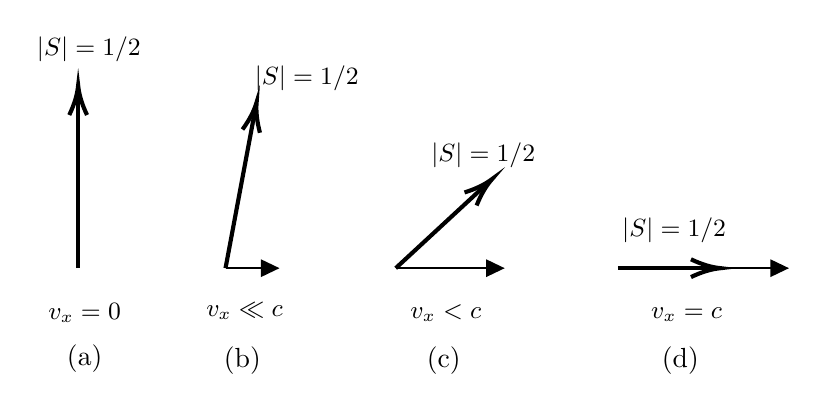
\begin{tikzpicture}[x=0.75pt,y=0.75pt,yscale=-1,xscale=1]
%uncomment if require: \path (0,300); %set diagram left start at 0, and has height of 300

%Straight Lines [id:da533603137195499] 
\draw [line width=1.5]    (79.87,190.5) -- (79.87,105.5) ;
\draw [shift={(79.87,102.5)}, rotate = 450] [color={rgb, 255:red, 0; green, 0; blue, 0 }  ][line width=1.5]    (14.21,-4.28) .. controls (9.04,-1.82) and (4.3,-0.39) .. (0,0) .. controls (4.3,0.39) and (9.04,1.82) .. (14.21,4.28)   ;

%Straight Lines [id:da31466198885223695] 
\draw    (150.87,190.5) -- (173.87,190.5) ;
\draw [shift={(176.87,190.5)}, rotate = 180] [fill={rgb, 255:red, 0; green, 0; blue, 0 }  ][line width=0.08]  [draw opacity=0] (8.93,-4.29) -- (0,0) -- (8.93,4.29) -- cycle    ;

%Straight Lines [id:da6431925700861189] 
\draw [line width=1.5]    (150.87,190.5) -- (165.31,113.45) ;
\draw [shift={(165.87,110.5)}, rotate = 460.62] [color={rgb, 255:red, 0; green, 0; blue, 0 }  ][line width=1.5]    (14.21,-4.28) .. controls (9.04,-1.82) and (4.3,-0.39) .. (0,0) .. controls (4.3,0.39) and (9.04,1.82) .. (14.21,4.28)   ;

%Straight Lines [id:da8282450907912188] 
\draw    (232.87,190.5) -- (282.37,190.5) ;
\draw [shift={(285.37,190.5)}, rotate = 180] [fill={rgb, 255:red, 0; green, 0; blue, 0 }  ][line width=0.08]  [draw opacity=0] (8.93,-4.29) -- (0,0) -- (8.93,4.29) -- cycle    ;

%Straight Lines [id:da09697600465348566] 
\draw [line width=1.5]    (232.87,190.5) -- (277.16,149.54) ;
\draw [shift={(279.37,147.5)}, rotate = 497.24] [color={rgb, 255:red, 0; green, 0; blue, 0 }  ][line width=1.5]    (14.21,-4.28) .. controls (9.04,-1.82) and (4.3,-0.39) .. (0,0) .. controls (4.3,0.39) and (9.04,1.82) .. (14.21,4.28)   ;

%Straight Lines [id:da13695386046952507] 
\draw    (339.87,190.5) -- (419.33,190.5) ;
\draw [shift={(422.33,190.5)}, rotate = 180] [fill={rgb, 255:red, 0; green, 0; blue, 0 }  ][line width=0.08]  [draw opacity=0] (8.93,-4.29) -- (0,0) -- (8.93,4.29) -- cycle    ;

%Straight Lines [id:da04790853968035602] 
\draw [line width=1.5]    (339.87,190.5) -- (386.33,190.5) ;
\draw [shift={(389.33,190.5)}, rotate = 180] [color={rgb, 255:red, 0; green, 0; blue, 0 }  ][line width=1.5]    (14.21,-4.28) .. controls (9.04,-1.82) and (4.3,-0.39) .. (0,0) .. controls (4.3,0.39) and (9.04,1.82) .. (14.21,4.28)   ;


% Text Node
\draw (85,85.07) node  [font=\small]  {$|S|=1/2$};
% Text Node
\draw (83,212.07) node  [font=\small]  {$v_{x} =0$};
% Text Node
\draw (160,211.07) node  [font=\small]  {$v_{x} \ll c$};
% Text Node
\draw (257,212.07) node  [font=\small]  {$v_{x} < c$};
% Text Node
\draw (373,213.07) node  [font=\small]  {$v_{x} =c$};
% Text Node
\draw (190,99.07) node  [font=\small]  {$|S|=1/2$};
% Text Node
\draw (275,136.07) node  [font=\small]  {$|S|=1/2$};
% Text Node
\draw (367,172.07) node  [font=\small]  {$|S|=1/2$};
% Text Node
\draw (83,234.07) node   [align=left] {(a)};
% Text Node
\draw (159,235.07) node   [align=left] {(b)};
% Text Node
\draw (256,235.07) node   [align=left] {(c)};
% Text Node
\draw (370,235.07) node   [align=left] {(d)};


\end{tikzpicture}

    \caption{Effect of Transverse Velocity on Dirac Particle Spin}
    \label{fig:transverse-velocity-effect}
\end{figure}

In general, for $j=a,b,c,d$, the four states shown (for a C type particle) in the figure are
\begin{equation}
\left|\psi_{(j)}\right\rangle=\sqrt{\frac{m}{V E_{p_{j}}}}\left(C_{1}\left(p_{j}\right) u_{1}\left(p_{j}\right)+C_{2}\left(p_{j}\right) u_{2}\left(p_{j}\right)\right) e^{-i p_{j} x}
\label{psi-abcd}
\end{equation}
Not that we have a particle here (so no $D$ type terms), and $\mathbf{p}_j$ is known. State (a) there is effectively spin up with $\mathrm{p}_{\mathrm{a}}=0$, so
\begin{equation}
\left|\psi_{(a)}\right\rangle=\sqrt{\frac{m}{V E_{p_{a}}}} C_{1}(0) u_{1}(0) e^{-i p_{a} x}=\sqrt{\frac{m}{V E_{\mathrm{p}_{a}}}} \sqrt{\frac{E_{\mathrm{p}_{a}}+m}{2 m}}\left(\begin{array}{l}
{\mathrm{I}} \\
{0} \\
{0} \\
{0}
\end{array}\right) e^{-i p_{a} x}
\end{equation}
which is an eigenstate of $\Sigma_3$. So for state (a), $|\psi_a\rangle$ has $C_1=1$ and $C_2=0$.

For the last state (d), where the particle is traveling at the speed of light, (\ref{psi-abcd}) becomes an eigenstate of $\Sigma_1$ with eigenvalue $1/2$,
$$
\left|\psi_{(d)}\right\rangle=\sqrt{\frac{m}{V E_{\mathrm{p}_{d}}}} C_{1}(\infty) u_{1}(\infty) e^{-i p_{d} x}+\sqrt{\frac{m}{V E_{\mathrm{p} d}}} C_{2}(\infty) u_{2}(\infty) e^{-i p_{d} x}
$$
$$
=\sqrt{\frac{m}{V E_{\mathrm{p}_{d}}}} \sqrt{\frac{E_{\mathrm{p}_{d}}+m}{2 m}}\left(\begin{array}{l}
{1} \\
{1} \\
{1} \\
{1}
\end{array}\right) e^{-i p_{d} x}
$$
where here, we must have $C_1=C_2=1$. (in the normalized version, $C_1=C_2=1/\sqrt{2}$).For "in between" states $(b)$ and $(c), C_{1}$ and $C_{2}$ would have other values. The bottumline is:\redp{$\mathbf{p}$ determines $u_{1,2}$ and then spin is represented by correct linear combination of $u_1$ and $u_2$}. Note that \bluep{we can never have a relativistic state where the spin vector and $\mathbf{p}$ are at right angles.}

Note that $u_{1}$ and $u_{2}$ actually exist in spinor space (they are spinor space basis vectors in that space), but they correspond to directions in physical space. For example, in the at-rest system, $u_1$ represents spin up and so can be visualized as a spatial vector that points in the $+z$ direction. Similarly, in the at-rest system, $u_{2}$ represents spin down, so can be visualized as a vector pointing in the $-z$ direction. 
\begin{qt}
\underline{Summary}

1. $u_{1}(\mathrm{p}) e^{-i p x}$ and  $u_{2}(\mathrm{p}) e^{-i p x}$ is each always an eigenstate of the Dirac equation (for any $\mathbf{p}$)

2. $u_{1}(\mathrm{p}) e^{-i p x}$ and $u_{2}(\mathrm{p}) e^{-i p x}$ is each sometimes an eigenstate of $z$ spin, i.e. of $\Sigma_{3}\left(\text { for } \mathbf{p}=0 \text { or }=p^{3} \mathbf{i}_{3}\right)$

3. $u_{1}(\mathbf{p}) e^{-i p x}$ and $u_{2}(\mathbf{p}) e^{-i p x}$ are always basis vectors for any general state $|\psi\rangle$ (for any $\mathbf{p}$ )

4. $u_{1}(p)$ and $u_{2}(p)$ is each sometimes an eigenstate of $z$ spin, i.e. of $\Sigma_{3}$ for $\mathbf{p}=0$ or$=p^{3} \mathbf{i}_{3}$)

5. $u_{1}(\mathbf{p})$ and $u_{2}(\mathbf{p})$ are always basis vectors in $4 \mathrm{D}$ spinor space (for any $\mathbf{p}$) 

6. \textbf{$u_{1}(\mathrm{p})$ and $u_{2}(\mathrm{p})$ change orientation, as visualized in physical space, as $\mathrm{p}$ changes.}

7. Spin S (often in relativity as $\Sigma$ ) changes direction with p, but differently than $u_{1}$ and $u_{2}$
\end{qt}
Any general spin state $u$ can be represented as a linear combination of $u_{1}$ and  $u_{2}$ (for any $\mathbf{p}$)
$$
u(\mathrm{p})=C_{1}(\mathrm{p}) u_{1}(\mathrm{p})+C_{2}(\mathrm{p}) u_{2}(\mathrm{p})
$$
Any general particle state includes a spin part plus a spacetime part(for any given $\mathbf{p}$):
$$
\left|\psi_{\mathfrak{p}}\right\rangle=\sqrt{\frac{m}{2 V E_{\mathrm{p}}}} u(\mathbf{p}) e^{-i p x}=\sqrt{\frac{m}{2 V E_{\mathrm{p}}}}\left(C_{1}(\mathrm{p}) u_{1}(\mathrm{p}) e^{-i p x}+C_{2}(\mathrm{p}) u_{2}(\mathrm{p}) e^{-i p x}\right)
$$
\subsection{RQM Helicity operator}
For massless particles ($v=c$), the velocity vector must perfectly align with the spin vector. This alignment is called \textbf{perfect helicity}. In general, if the spin axis (using the right-hand rule), of a particle is in the direction of $v$ one
says the particle has \textbf{positive helicity}. If spin points in the direction of $- v$, the particle has \textbf{negative helicitv}. 

The degree  of helicity a particle has be define in terms of the angle between the spin vector and the velocity vector. It is maximum if that angle is zero.\textbf{ The dot product of the spin vector with a unit vector in the $\mathbf{p}$ (or equivalently, the $v$) direction has come to be the mathematical definition of helicity}.

\bluep{Our spin operator $\Sigma$ in RQM plays the role of a 3-vector in physical space that points in the direction of spin.} The inner product in physical space of the spin operator $\Sigma$ and the unit vector in the $\mathbf{p}$ direction would then be \textbf{helicity operator}:
\begin{qt}
\begin{equation}
\Sigma_{p}=\Sigma \cdot i_{p}=\Sigma \cdot \frac{p}{|p|}=\Sigma_{1} \frac{p^{1}}{|p|}+\Sigma_{2} \frac{p^{2}}{|p|}+\Sigma_{3} \frac{p^{3}}{|p|}
\label{helicity-operator}
\end{equation}
(\ref{helicity-operator}) is a $4\times4$ matrix in spinor space because each $\Sigma_i$ is a matrix. (\ref{helicity-operator}) is a scalar in physical space because it is the inner product of two vectors.
\end{qt}
\begin{example}
Consider a case where a particle is in the first eigenstate of (\ref{four-spinors}), and if $p^3\neq0$, we have
$$
\Sigma \cdot \frac{\mathbf{p}}{|\mathbf{p}|}\left|\psi^{(1)}\right\rangle=\Sigma_{3} \underbrace{\frac{p^{3}}{|\mathbf{p}|}}_{=1}\left|\psi^{(1)}\right\rangle=\frac{1}{2}\left[\begin{array}{cccc}
{1} \\
{} & {-1} \\
{} & {} & {1} \\
{} & {} & {} & {-1}
\end{array}\right]\sqrt{\frac{E+m}{2 m}}\left(\begin{array}{c}
{1} \\
{0} \\
{\frac{p^3}{E+m}} \\
{0}
\end{array}\right)e^{-ipx}=\frac{1}{2}\left|\psi^{(1)}\right\rangle
$$
\end{example}
\begin{example}
Note that if $p^3$ were negative (-z direction)
$$
\Sigma_{3}\left|\psi^{(1)}\right\rangle=\frac{1}{2}\left[\begin{array}{cccc}
{1} \\
{} & {-1} \\
{} & {} & {1} \\
{} & {} & {} & {-1}
\end{array}\right]\sqrt{\frac{E+m}{2 m}}\left(\begin{array}{c}
{1} \\
{0} \\
{\frac{p^{3}}{E+m}} \\
{0}
\end{array}\right) e^{-i p x}=\frac{1}{2}\left|\psi^{(1)}\right\rangle
$$
but
$$
\Sigma \cdot \frac{\mathbf{p}}{|\mathbf{p}|}\left|\psi^{(1)}\right\rangle=\Sigma_{3} \underbrace{\frac{p^{3}}{|\mathbf{p}|}}_{=-1}\left|\psi^{(1)}\right\rangle=-\frac{1}{2}\left|\psi^{(1)}\right\rangle
$$
\end{example}
In general, a $+1 / 2$ helicity state for spinors means the spin is in the direction of $p$; a $-1 / 2$ helicity eigenvalue means spin is in the direction of $-p$.

\section{The Dirac Equation in QFT}
The Dirac equation for fields (where we will, as with scalar fields, work in the Heisenberg picture), is
\begin{equation}
\left(i \gamma^{\mu} \partial_{\mu}-m\right) \psi=0
\end{equation}
Its eigensolutions
\begin{equation}
\psi^{(1)}=u_{1} e^{-i p x} \quad \psi^{(2)}=u_{2} e^{-i p x} \quad \psi^{(3)}=v_{2} e^{i p x} \quad \psi^{(4)}=v_{1} e^{i p x}
\end{equation}
\textbf{\underline{The adjoint Dirac equation for fields is}}
\begin{equation}
i \partial_{\mu} \bar{\psi} \gamma^{\mu}+m \bar{\psi}=0
\end{equation}
with adjoint eigensolutions
\begin{equation}
\bar{\psi}=\psi^{\dagger} \gamma^{0} \rightarrow \bar{\psi}^{(1)}=u_{1}^{\dagger} \gamma_{e}^{0} e^{i p x}=\bar{u}_{\mathrm{l}} e^{i p x} \quad \bar{\psi}^{(2)}=\bar{u}_{2} e^{i \phi x} \quad \bar{\psi}^{(3)}=\bar{v}_{2} e^{-i \varphi x} \quad \bar{\psi}^{(4)}=\bar{v}_{1} e^{-\dot{\varphi} x}
\end{equation}
\begin{qt}
the general discrete plane wave solutions are
\begin{equation}
\begin{aligned}
\psi &=\sum_{r, \mathbf{p}} \sqrt{\frac{m}{V E_{\mathrm{p}}}}\left(c_{r}(\mathbf{p}) u_{r}(\mathbf{p}) e^{-i p x}+d_{r}^{\dagger}(\mathbf{p}) v_{r}(\mathbf{p}) e^{i p x}\right) \\
&=\quad \psi^{+} \quad+\quad \psi^{-}
\end{aligned}
\end{equation}
\begin{equation}
\begin{aligned}
&\bar{\psi}=\sum_{r, p} \sqrt{\frac{m}{V E_{p}}}\left(d_{r}(p) \bar{v}_{r}(p) e^{-i p x}+c_{r}^{\dagger}(p) \bar{u}_{r}(p) e^{i p x}\right)\\
&=\quad \bar{\psi}^{+} \quad+\quad \bar{\psi}^{-}
\end{aligned}
\end{equation}
\end{qt}
The general continuous plane wave solutions are
\begin{equation}
\begin{aligned}
&\psi=\sum_{r} \sqrt{\frac{m}{(2 \pi)^{3}}} \int \frac{d^{3} \mathbf{p}}{\sqrt{E_{p}}}\left(c_{r}(\mathbf{p}) u_{r}(\mathbf{p}) e^{-i p x}+d_{r}^{\dagger}(\mathbf{p}) v_{r}(\mathbf{p}) e^{i p x}\right)\\
&\bar{\psi}=\sum_{r} \sqrt{\frac{m}{(2 \pi)^{3}}} \int \frac{d^{3} \mathbf{p}}{\sqrt{E_{p}}}\left(d_{r}(\mathbf{p}) \bar{v}_{r}(\mathbf{p}) e^{-i p x}+c_{r}^{\dagger}(\mathbf{p}) \bar{u}_{r}(\mathbf{p}) e^{i p x}\right)
\end{aligned}
\end{equation}
\begin{qt}
the Lagrangian ( density) for free spinor fields to be
\begin{equation}
\mathcal{L}_{0}^{1/2}=\bar{\psi}\left(i \gamma^{\alpha} \partial_{\alpha}-m\right) \psi
\end{equation}
Conjugate momenta for $\psi$ and $\bar{\psi}$ are
\begin{equation}
\pi^{1 / 2}=\frac{\partial \mathcal{L}_{0}^{1 / 2}}{\partial \psi_{0}}=i \psi \gamma^{0}=i \psi^{\dagger} \gamma^{\dagger} \gamma^{0}=i \psi^{\dagger}
\end{equation}
\begin{equation}
\bar{\pi}^{1 / 2}=\frac{\partial \mathcal{L}_{0}^{1 / 2}}{\partial \bar{\psi}_{, 0}}=0
\end{equation}
The Dirac Hamiltonian density can be found from the Legendre transformation as
\begin{equation}
\begin{aligned}
\mathcal{H}_{0}^{1 / 2} &=\pi^{1 / 2} \dot{\psi}+\bar{\pi}^{1 / 2} \dot{\bar{\psi}}-\mathcal{L}_{0}^{1 / 2}=i \psi^{\dagger} \dot{\psi}-\mathcal{L}_{0}^{1 / 2}=i \underbrace{\psi^{\dagger} \gamma^{0}}_{\bar{\psi}} \gamma^{0} \dot{\psi}-\mathcal{L}_{0}^{1 / 2} \\
&=i \bar{\psi} \gamma^{0} \dot{\psi}\underbrace{-i \bar{\psi} \gamma^{0} \dot{\psi}-i \bar{\psi} \gamma^{i} \partial_{i} \psi}_{-i\bar{\psi}\gamma^{\alpha}\partial_{\alpha}\psi}+m \bar{\psi} \psi=-i \bar{\psi} \gamma^{i} \partial_{i} \psi+m \bar{\psi} \psi
\end{aligned}
\end{equation}
\end{qt}
\section{Anti-commutation Relations for Dirac Fields}
\begin{qt}
\begin{equation}
    \left[c_{r}(\mathbf{p}), c_{s}^{\dagger}\left(\mathbf{p}^{\prime}\right)\right]_{+}=\left[d_{r}(\mathbf{p}), d_{s}^{\dagger}\left(\mathbf{p}^{\prime}\right)\right]_{+}=\delta_{r S} \delta_{\mathbf{p p}^{\prime}}(\text { discrete }) ;=\delta_{r s} \delta(\mathbf{p - p ^ { \prime }})(\text { continuous })
\end{equation}
All other anti-commutators between coefficients equal zero.
\end{qt}
\section{The Dirac Hamiltonian in QFT}
Similar to what we did for scalar fields, we find the Dirac Hamiltonian by integrating the Dirac Hamiltonian density over all space (a volume V containing the discrete solutions, which we can make as large as we like), i.e.,
\begin{equation}
H_{0}^{1 / 2}=\int \mathcal{H}_{0}^{1 / 2} d^{3} x=\int\left(-i \bar{\psi} \gamma^{i} \partial_{i} \psi+m \bar{\psi} \psi\right) d^{3} x
\label{Dirac-Hamiltonian}
\end{equation}
we substitute the Dirac general solution into (\ref{Dirac-Hamiltonian}) to give
$$
\begin{aligned}
&H_{0}^{1 / 2}=\int\left(-i \bar{\psi} \gamma^{i} \partial_{i} \psi+m \bar{\psi} \psi\right) d^{3} x=\\
&\int\left(\sum_{r, p} \sqrt{\frac{m}{V E_{p}}}\left(d_{r}(p) \bar{v}_{r}(\mathbf{p}) e^{-i p x}+c_{r}^{\dagger}(\mathbf{p}) \bar{u}_{r}(\mathbf{p}) e^{i p x}\right)\right) \times
\end{aligned}
$$
$$
\left(-i \gamma^{i} \partial_{i}\right)\left(\sum_{s, p^{\prime}} \sqrt{\frac{m}{V E_{p^{\prime}}}}\left(c_{s}\left(\mathbf{p}^{\prime}\right) u_{s}\left(\mathbf{p}^{\prime}\right) e^{-i p^{\prime} x}+d_{s}^{\dagger}\left(\mathbf{p}^{\prime}\right) v_{s}\left(\mathbf{p}^{\prime}\right) e^{i p^{\prime} x}\right)\right) d^{3} x
$$
$$
+\int m\left(\sum_{r, p} \sqrt{\frac{m}{V E_{p}}}\left(d_{r}(p) \bar{v}_{r}(p) e^{-i p x}+c_{r}^{\dagger}(p) \bar{u}_{r}(p) e^{i p x}\right)\right) \times
$$
$$
\left(\sum_{s, \mathbf{p}^{\prime}} \sqrt{\frac{m}{V E_{\mathbf{p}^{\prime}}}}\left(c_{s}\left(\mathbf{p}^{\prime}\right) u_{s}\left(\mathbf{p}^{\prime}\right) e^{-i p^{\prime} x}+d_{s}^{\dagger}\left(\mathbf{p}^{\prime}\right) v_{s}\left(\mathbf{p}^{\prime}\right) e^{i \mathbf{p}^{\prime} \cdot x}\right)\right) d^{3} x
$$
The first of the two integrals above becomes
$$
 \int\left(\sum_{r, \mathbf{p}} \sqrt{\frac{m}{V E_{p}}}d_{r}(\mathbf{p}) \bar{v}_{r}(\mathbf{p}) e^{-i\left(E_{p} t-p^{i} x^{i}\right)}\right)\left(\sum_{s, p^{\prime}} \sqrt{\frac{m}{V E_{p^{\prime}}}} c_{s}\left(\mathbf{p}^{\prime}\right) \gamma^{i} \underbrace{p^{\prime i}}_{\text { from }\partial_i} u_{s}\left(\mathbf{p}^{\prime}\right) e^{-i\left(E_{p^{\prime}}-p^{\prime i} x^{i}\right)}\right)d^3x
$$
$$
+\int\left(\sum_{r, \mathrm{p}} \sqrt{\frac{m}{V E_{\mathrm{p}}}} d_{r}(\mathrm{p}) \bar{v}_{r}(\mathbf{p}) e^{-i\left(E_{\mathrm{p}} t-p^{i} x^{i}\right)}\right)\left(\sum_{s, p^{\prime}} \sqrt{\frac{m}{V E_{p^{\prime}}}} d_{s}^{\dagger}\left(p^{\prime}\right) \gamma^{i}\left(-p^{\prime i}\right) v_{s}\left(p^{\prime}\right) e^{i\left(E_{p^{\prime}}t-p^{\prime i} x^{i}\right)}\right) d^{3} x
$$
$$
+\int\left(\sum_{r, \mathrm{p}} \sqrt{\frac{m}{V E_{\mathrm{p}}}} c^{\dagger}_{r}(\mathrm{p}) \bar{u}_{r}(\mathbf{p}) e^{-i\left(E_{\mathrm{p}} t-p^{i} x^{i}\right)}\right)\left(\sum_{s, p^{\prime}} \sqrt{\frac{m}{V E_{p^{\prime}}}} c_{s}\left(p^{\prime}\right) \gamma^{i}\left(p^{\prime i}\right) u_{s}\left(p^{\prime}\right) e^{i\left(E_{p^{\prime}}t-p^{\prime i} x^{i}\right)}\right) d^{3} x
$$
$$
+\int\left(\sum_{r, \mathrm{p}} \sqrt{\frac{m}{V E_{\mathrm{p}}}} c^{\dagger}_{r}(\mathrm{p}) \bar{u}_{r}(\mathbf{p}) e^{-i\left(E_{\mathrm{p}} t-p^{i} x^{i}\right)}\right)\left(\sum_{s, p^{\prime}} \sqrt{\frac{m}{V E_{p^{\prime}}}} d^{\dagger}_{s}\left(p^{\prime}\right) \gamma^{i}\left(-p^{\prime i}\right) v_{s}\left(p^{\prime}\right) e^{i\left(E_{p^{\prime}}t-p^{\prime i} x^{i}\right)}\right) d^{3} x
$$
\redp{because an integral over all space of the oscillating function $e^{if(\mathbf{x})}$, where $f(\mathbf{x}\neq0)$ is zero. }So,in the first and last lines, only terms with $\mathbf{p}=-\mathbf{p}^{\prime}$ will survive. And in the $2^{\text {nd }}$ and $3^{\text {rd }}$ lines, only terms in $\mathbf{p}^{\prime}=\mathbf{p}$ will. We assume, as in $\mathrm{RQM},$ that \textbf{\redp{the order of spinors and coefficients (such as $c_{r} \text { and } d_{r}$) can be interchanged at will, but we must preserve the order of spinor entities as it represent matrix/vector multiplication in spinor space.}}
$$
+\int\left[\sum_{r, s, \mathbf{p}} \frac{m}{V E_{\mathbf{p}}} d_{r}(-\mathbf{p}) \bar{v}_{r}(-\mathbf{p}) \gamma^{i} p^{i} u_{s}(\mathbf{p}) c_{s}(\mathbf{p}) e^{-i 2 E_{p} t}\right] d^{j}
$$
$$
+\int\left(\sum_{r, s, \mathbf{p}} \frac{m}{V E_{\mathrm{p}}} d_{r}(\mathbf{p}) \bar{v}_{r}(\mathbf{p}) \gamma^{i}\left(-p^{i}\right) v_{s}(\mathbf{p}) d_{s}^{\dagger}(\mathbf{p})\right) d^{3} x
$$
$$
+\int\left(\sum_{r, s, \mathbf{p}} \frac{m}{V E_{p}} c_{r}^{\dagger}(\mathbf{p}) \bar{u}_{r}(\mathbf{p}) \gamma^{i} p^{i} u_{s}(\mathbf{p}) c_{s}(\mathbf{p})\right) d^{3} x
$$
$$
+\int\left(\sum_{r, s, \mathbf{p}} \frac{m}{V E_{p}} c_{r}^{\dagger}(-\mathbf{p}) \bar{u}_{r}(-\mathbf{p}) \gamma^{i}\left(-p^{i}\right) v_{s}(\mathbf{p}) d_{s}^{\dagger}(\mathbf{p}) e^{i 2 E_{p} t}\right) d^{3} x
$$
In similar fashion. the last two lines of the expansion of (\ref{Dirac-Hamiltonian}), representing the mass term in $H^{1/2}_0$, become
$$
\int\left(\sum_{r, s, \mathbf{p}} \frac{m}{V E_{p}} d_{r}(-\mathbf{p}) \bar{v}_{r}(-\mathbf{p}) m u_{s}(\mathbf{p}) c_{s}(\mathbf{p}) e^{-i 2 E_{p} t}\right) d^{3} x
$$
$$
\begin{aligned}
&+\int\left(\sum_{r, s, \mathbf{p}} \frac{m}{V E_{\mathbf{p}}} d_{r}(\mathbf{p}) \bar{v}_{r}(\mathbf{p}) m v_{s}(\mathbf{p}) d_{s}^{\dagger}(\mathbf{p})\right) d^{3} x\\
&+\int\left(\sum_{r, s, \mathbf{p}} \frac{m}{V E_{\mathrm{p}}} c_{r}^{\dagger}(\mathbf{p}) \bar{u}_{r}(\mathbf{p}) m u_{s}(\mathbf{p}) c_{s}(\mathbf{p})\right) d^{3} x
\end{aligned}
$$
$$
+\int\left(\sum_{r, s, \mathbf{p}} \frac{m}{V E_{\mathbf{p}}} c_{r}^{\dagger}(-\mathbf{p}) \bar{u}_{r}(-\mathbf{p}) m v_{s}(\mathbf{p}) d_{s}^{\dagger}(\mathbf{p}) e^{i 2 E_{\mathbf{p}} t}\right) d^{3} x
$$
\begin{mybox}
\textbf{Relationship for $u_{s}(\mathbf{p})$}

Consider the Dirac equation and a single eigensolution to it having 3 -momentum p and spin $s$
$$
\left(i \gamma^{\mu} \partial_{\mu}-m\right) \psi=(i \not \partial-m) \psi=0 \quad \text { with } \quad \psi=c_{\underline{s}}(\mathbf{p}) u_{\underline{s}}(\mathbf{p}) e^{-i p x}
$$
$$
\left(\gamma^{\mu} p_{\mu}-m\right) c_{\underline{s}}(\mathbf{p}) u_{\underline{s}}(\mathbf{p}) e^{-i p x}=(\not p-m) c_{\underline{s}}(\mathbf{p}) u_{\underline{s}}(\mathbf{p}) e^{-i p x}=0
$$
\textbf{Neither $c_{s}(p)$ nor the exponential equal zero, so the remaining factors must equal zero}, thus
$$
\left(\gamma^{\mu} p_{\mu}-m\right) u_{s}(\mathbf{p})=(\not p-m) u_{s}(\mathbf{p})=0
$$
Now from the complex conjugate transpose of (\ref{coefficient-orthogonality}), where r and s are dummy variables and thus interchangeable and the relation holds for any $\mathbf{p}$, including $-\mathbf{p}$,
$$
\begin{aligned}
u_{r}^{\dagger}(\mathbf{p}) v_{s}(-\mathbf{p})=0 & \rightarrow v_{s}^{\dagger}(-\mathbf{p}) u_{r}(\mathbf{p})=0 \rightarrow v_{r}^{\dagger}(-\mathbf{p}) u_{s}(\mathbf{p})=0 \\
v_{r}^{\dagger}(-\mathbf{p}) \gamma^{0} \gamma^{0} u_{s}(\mathbf{p})=0 & \rightarrow \bar{v}_{r}(-\mathbf{p}) \gamma^{0} u_{s}(\mathbf{p})=0 \rightarrow \bar{v}_{r}(-\mathbf{p}) \gamma^{0} p_{0} u_{s}(\mathbf{p})=0
\end{aligned}
$$
And thus,
$$
\bar{v}_{r}(-\mathrm{p}) \gamma^{i} p^{i} u_{s}(\mathrm{p})=\bar{v}_{r}(-\mathrm{p}) \gamma^{i}\left(-p_{i}\right) u_{s}(\mathrm{p})-\bar{v}_{r}(-\mathrm{p}) \gamma^{0} p_{0} u_{s}(\mathrm{p})=-\bar{v}_{r}(-\mathrm{p}) \underbrace{\gamma^{\mu} p_{\mu}}_{\not p} u_{s}(\mathrm{p})
$$
When we then use the RHS instead of the LHS of the equation above, we get
$$
-\int\left(\sum_{r, s, \mathbf{p}} \frac{m}{V E_{\mathbf{p}}} d_{r}(-\mathbf{p})(\bar{v}_{r}(-\mathbf{p})\underbrace{(\not p-m)u_s(\mathbf{p})}_{=0} c_{s}(\mathbf{p}) e^{-i 2 E_{p} t}\right) d^{3} x=0
$$
\end{mybox}
Recall that 
$$
v_{r}^{\dagger}(\mathbf{p}) v_{s}(\mathbf{p})=\bar{v}_{r}(\mathbf{p}) \gamma^{0} v_{s}(\mathbf{p})=\frac{E_{p}}{m} \delta_{r s}=\frac{p_{0}}{m} \delta_{r s}
$$
we have
$$
\bar{v}_{r}(\mathbf{p}) \gamma^{0} p_{0} v_{s}(\mathbf{p})=\frac{\left(p_{0}\right)^{2}}{m} \delta_{r s}=\frac{E_{p}^{2}}{m} \delta_{r s}
$$
Adding the integrals above, and using the relationship in the box, we find
\begin{equation}
\begin{aligned}
&\int\left(\sum_{r, s, \mathbf{p}} \frac{m}{V E_{p}} d_{r}(\mathbf{p}) \bar{v}_{r}(\mathbf{p})\left(-\gamma^{i} p^{i}+m\right) v_{s}(\mathbf{p}) d_{s}^{\dagger}(\mathbf{p})\right) d^{3} x\\
&=\int\left(\sum_{r \leq p} \frac{m}{V E_{p}} d_{r}(p)\left(\bar{v}_{r}(p)\left(\gamma^{i} p_{i}+m+\gamma^{0} p_{0}\right) v_{s}(p)-\frac{E_{p}^{2}}{m} \delta_{r s}\right) d_{s}^{\dagger}(p)\right) d^{3} x\\
&=\frac{1}{V} \int_{=1}^{1} d^{3} x\left(\sum_{r,s, p} \frac{m}{E_{p}} d_{r}(p)\left(\gamma^{\mu} p_{\mu}+m\right){v_{s}(p)-\frac{E_{p}^{2}}{m} \delta_{r s}}\right) d_{s}^{\dagger}(p)
\end{aligned}
\end{equation}
Note that $(\not p+m) v_{s}(p)=0$, the equation above reduces to
\begin{equation}
\sum_{r, \mathrm{p}} \frac{m}{E_{\mathrm{p}}} d_{r}(\mathbf{p})\left(-\frac{E_{\mathrm{p}}^{2}}{m}\right) d_{r}^{\dagger}(\mathbf{p})=-\sum_{r, \mathbf{p}} E_{\mathbf{p}} \underbrace{d_{r}(\mathbf{p}) d_{r}^{\dagger}(\mathbf{p})}_{\text {use anti-commutator }}
\end{equation}
Finally,
\begin{qt}
\begin{equation}
H_{0}^{1 / 2}=\sum_{r, p} E_{p}\left(N_{r}(p)-\frac{1}{2}+\bar{N}_{r}(p)-\frac{1}{2}\right)
\end{equation}
\begin{equation}
N_{r}(\mathbf{p})=c_{\underline{r}}^{\dagger}(\mathbf{p}) c_{\underline{r}}(\mathbf{p}) \quad \bar{N}_{r}(\mathbf{p})=d_{\underline{r}}^{\dagger}(\mathbf{p}) d_{\underline{r}}(\mathbf{p}) \quad \text { (underbars mean no summation) }
\end{equation}
where

$N_{r}(\mathbf{p})=$ number operator with eigenvalue $n_{r}(\mathbf{p})=$ number of $c$ particles of 3 -mom $\mathbf{p},$ spin $r$ in the ket,

$\bar{N}_{r}(\mathbf{p})=$ number operator with eigenvalue $\bar{n}_{r}(\mathbf{p})=$ number of $d$ particles with $\mathbf{p}$ and spin $r$ in the ket,

and, the vacuum has $-1 / 2$ quantum of energy for each $\mathrm{p}, r$ for $c$ particles, and also for $d$ particles
\end{qt}
Note that
\begin{equation}
H_{0}^{1 / 2}|0\rangle=\sum_{r, p} E_{p}\left(N_{r}(p)-\frac{1}{2}+\bar{N}_{r}(p)-\frac{1}{2}\right)|0\rangle=\sum_{r, p} E_{p}\left(-\frac{1}{2}-\frac{1}{2}\right)|0\rangle
\end{equation}
\textbf{This infinite negative energy indicates that there is still something missing from the extant theory.}

\section{Creation and Destruction Operators}
It will probably not come as a big surprise that the $c_{r}(\mathbf{p})$ and $d_{r}(\mathbf{p})$ operators destroy Dirac particles, and their complex conjugates create Dirac particles. We prove this below.

From the anti-commutation relations,
\begin{equation}
\left[c_{r}^{\dagger}(\mathbf{p}), c_{r}^{\dagger}(\mathbf{p})\right]_{+}=\left[c_{r}(\mathbf{p}), c_{r}(\mathbf{p})\right]_{+}=0
\end{equation}
Thus,
\begin{equation}
c_{r}^{\dagger}(\mathbf{p}) c_{r}^{\dagger}(\mathbf{p})+c_{r}^{\dagger}(\mathbf{p}) c_{r}^{\dagger}(\mathbf{p})=0 \rightarrow\left(c_{r}^{\dagger}(\mathbf{p})\right)^{2}=0
\end{equation}
Similarly
$$\left(c_{r}(\mathbf{p})\right)^{2}=0 \quad\left(d_{r}^{\dagger}(\mathbf{p})\right)^{2}=0\quad \left(d_{r}(p)\right)^{2}=0
$$
\underline{Proof that $c_r(\mathbf{p})$ is a Destruction operator}
$$
c_{r}(\mathbf{p})\left|\psi_{r . p}\right\rangle=|?\rangle
$$
Use the number operator, we have
$$
N_{r}(\mathbf{p})|?\rangle= n_{?}|?\rangle= n_{?} c_{r}(\mathbf{p})\left|\psi_{r, \mathbf{p}}\right\rangle=\left(1-c_{r}(\mathbf{p}) c_{r}^{\dagger}(\mathbf{p})\right) c_{r}(\mathbf{p})\left|\psi_{r, \mathbf{p}}\right\rangle
$$
$$
=c_{I}(\mathbf{p})\left|\psi_{r, \mathbf{p}}\right\rangle- c_{r}(\mathbf{p}) \underbrace{n_{r}(\mathbf{p})}_{=1}\left|\psi_{r, \mathbf{p}}\right\rangle=(1-1) \underbrace{c_{r}(\mathbf{p})\left|\psi_{r, \mathbf{p}}\right\rangle}_{|?\rangle}
$$
When $c_r^{\dagger}(\mathbf{p})$ acts on a single particle state, we find
\begin{qt}
\begin{equation}
c_{r}^{\dagger}(\mathbf{p}) \underbrace{\left|\psi_{r, \mathbf{p}}\right\rangle}_{c_{r}^{\dagger}(\mathbf{p})|0\rangle}=\left(c_{r}^{\dagger}(\mathbf{p})\right)^{2}|0\rangle= 0
\end{equation}
So, the theory we've developed tells us that we cannot create (we cannot have) multiparticle with more than one Dirac particle in a given single particle state.
\end{qt}
\bluep{\textbf{General rule}}

Coefficient commutation relations work for bosons and allow more than one identical single particle state to $\mathrm{co}$ -exist in the same multiparticle state.

Coefficient anti-commutation relations work for fermions and do not allow more than one identical single particle state to co-exist in the same multiparticle state.

\subsection{Total Particle number}
As with scalars, total particle rtl.llilber is defined as the number of particles (i.e. c types) minus the number of antiparticles (d types). For spinors, the total particle number operator is
\begin{equation}
N(\psi)=\sum_{r, p}\left(N_{r}(\mathbf{p})-\bar{N}_{r}(\mathbf{p})\right)
\end{equation}
\textbf{Again, note the subtle difference in phraseology. "Number of particles" (which is different from "total particle number") equals the number of particles plus the number of antiparticles.}

\section{QFT Spinor Charge Operator and Four Current}
From what we know about the number operators, and parallel to what we found for scalar fields, we can simply define our Dirac charge operator as
\begin{qt}
\begin{equation}
Q=-e \sum_{r, p}\left(N_{r}(\mathbf{p})-\bar{N}_{r}(\mathbf{p})\right)
\label{Dirac-charge-operator}
\end{equation}
\end{qt}
Where - e is the charge on the electron. Note that, with this definition, d type particles will ~ave a
charge of+ e, which would qualify them as antiparticles of the electron. Note the operation of
(\ref{Dirac-charge-operator})on a typical state
$$
-e \sum_{r, \mathbf{p}}\left(N_{r}(\mathbf{p})-\bar{N}_{r}(\mathbf{p})\right)\left|\psi_{n, \mathbf{p}_{1}}, \psi_{n, \mathbf{p}_{2}}, \bar{\psi}_{n, \mathbf{p}_{1}}\right\rangle=\underbrace{-e(1+1-1)}_{\text { to charge }=-e}\left|\psi_{n, \mathbf{p}_{1},} \psi_{n, \mathbf{p}_{2}}, \bar{\psi}_{n, \mathbf{p}_{1}}\right\rangle
$$
A state With two electrons and one positron has a total charge Of -e.
\subsection{The Dirac charge operator from the four current}
\begin{qt}
\begin{equation}
\text { spinor 4-current operator } j^{\mu}=(\rho, \mathbf{j})=\bar{\psi} \gamma^{\mu} \psi \quad \text { with } \quad \partial_{\mu} j^{\mu}=0
\end{equation}
\end{qt}
\section{Dirac Three Momentum Operator}
we can simply define our Dirac 3-momentum operator as
\begin{equation}
\mathbf{P}=\sum_{r, \mathbf{p}} \mathbf{p}\left(N_{r}(\mathbf{p})+\bar{N}_{r}(\mathbf{p})\right)
\end{equation}
\section{Dirac Spin Operator in QFT}
\begin{qt}
We can define the \textbf{QFT Dirac spin operator} as
\begin{equation}
{}_\mathrm{QFT}{\Sigma_{i}}=\int_{V} \psi^{\dagger} \Sigma_{i} \psi d^{3} x \rightarrow \quad {}_\mathrm{QFT}{\Sigma_{3}}=\int_{V} \psi^{\dagger} \Sigma_{3} \psi d^{3} x
\end{equation}
\end{qt} 
For type c particles, we have
\begin{equation}
{}_{ QFT }{}^{c} \Sigma_{3}=\int_{V}\left(\sum_{r, p} \sqrt{\frac{m}{V E_{\mathbf{p}}}} c_{r}^{\dagger}(\mathbf{p}) u_{r}^{\dagger}(\mathbf{p}) e^{i p x}\right) \Sigma_{3}\left(\sum_{s, \mathbf{p}^{\prime}} \sqrt{\frac{m}{V E_{\mathbf{p}^{\prime}}}} c_{s}\left(\mathbf{p}^{\prime}\right) u_{s}\left(\mathbf{p}^{\prime}\right) e^{-i p^{\prime} x}\right) d^{3} x
\end{equation}
As we should be getting used to by now, all terms where $\mathbf{p} \neq \mathbf{p}^{\prime}$ will go to zero in the integration. giving us
\begin{equation}
{}_{ QFT }{}^{c} \Sigma_{3}=\left(\sum_{r, s, \mathrm{p}} c_{r}^{\dagger}(\mathbf{p}) c_{s}(\mathbf{p}) u_{r}^{\dagger}(\mathbf{p}) \Sigma_{3} u_{s}(\mathbf{p})\right) \frac{1}{V} \int d^{3} x=\left(\sum_{r, s, \mathbf{p}} u_{r}^{\dagger}(\mathbf{p}) \Sigma_{3} u_{s}(\mathbf{p}) c_{r}^{\dagger}(\mathbf{p}) c_{s}(\mathbf{p})\right)
\end{equation}
For a single particle state of spin s, the c operators will destroy that state, then create ones of spins r, i.e.,
\begin{equation}
\left(\sum_{r, s^{\prime}, p^{\prime}} \frac{m}{E_{p^{\prime}}} u_{r}^{\dagger}\left(\mathbf{p}^{\prime}\right) \Sigma_{3} u_{s^{\prime}}\left(\mathbf{p}^{\prime}\right) c_{r}^{\dagger}\left(\mathbf{p}^{\prime}\right) c_{s^{\prime}}\left(\mathbf{p}^{\prime}\right)\right) \left| \psi_{s, \mathbf{p}}\right\rangle=\sum_{r} \frac{m}{E_{\mathbf{p}}} \underbrace{\left(u_{r}^{\dagger}(\mathbf{p}) \Sigma_{3} u_{s}(\mathbf{p})\right)}_{\text {a number }}\left|\psi_{r, \mathbf{p}}\right\rangle
\end{equation}
So, the expectation value of what we would measure for spin in the z direction for the given state with s spin would be
$$
\left\langle\psi_{s, \mathrm{p}}\left|{}_{QFT}{}^{c} \Sigma_{3}\right| \psi_{s, \mathbf{p}}\right\rangle=\sum_{r} \frac{m}{E_{p}}\left\langle\psi_{s, p}\right|(\text { a number })\left|\psi_{r, \mathbf{p}}\right\rangle
$$
$$
=0 \text { for } r \neq s ; \quad=\frac{m}{E_{\mathrm{p}}} u_{r}^{\dagger}(\mathbf{p}) \Sigma_{3} u_{r}(\mathbf{p}) \text { for } r=s
$$
All of the above steps can be repeated analogously for $\Sigma_1$ and $\Sigma_2$ to yield the general result
\begin{qt}
\begin{equation}
{}_{QFT}{}^{c} \Sigma_{i}=\sum_{r, \mathrm{p}} \frac{m}{E_{\mathrm{p}}} u_{r}^{\dagger}(\mathbf{p}) \Sigma_{i} u_{r}(\mathbf{p}) N_{r}(\mathbf{p})
\end{equation}
For both type c and d particles
\begin{equation}
{}_{QFT}{}^{d} \Sigma_{i}=\left(\sum_{r, \mathrm{p}} \frac{m}{E_{\mathrm{p}}} v_{r}^{\dagger}(\mathbf{p}) \Sigma_{i} v_{r}(\mathbf{p}) \bar{N}_{r}(\mathbf{p})\right)
\end{equation}
Thus, \textbf{QFT spin operator in terms of number operators is}
\begin{equation}
{}_{QFT} \Sigma_{i}\sum_{r, \mathbf{p}} \frac{m}{E_{\mathbf{p}}}\left(u_{r}^{\dagger}(\mathbf{p}) \Sigma_{i} u_{r}(\mathbf{p}) N_{r}(\mathbf{p})+v_{r}^{\dagger}(\mathbf{p}) \Sigma_{i} v_{r}(\mathbf{p}) \bar{N}_{r}(\mathbf{p})\right)
\end{equation}
\end{qt}
\section{QFT Helicity Operator}
\begin{equation}
{}_{QFT} \Sigma_{\mathbf{p}}=\sum_{r, \mathbf{p}} \frac{m}{E_{\mathbf{p}}}\left(u_{r}^{\dagger}(\mathbf{p}) \Sigma_{i} \frac{p^{i}}{p} u_{r}(\mathbf{p}) N_{r}(\mathbf{p})+v_{r}^{\dagger}(\mathbf{p}) \Sigma_{i} \frac{p^{\prime}}{p} v_{r}(\mathbf{p}) \bar{N}_{r}(\mathbf{p})\right)
\end{equation}
\section{Anti-commutators are Outer Products}
For products of two fields, when the adjoint field is on the left and spinor indices are suppressed, an inner product is implied. Thus, where, as always, repeated indices mean summation,
\begin{equation}
\bar{\psi} \psi=\bar{\psi}_{\beta} \psi_{\beta}=\psi_{\alpha}^{\dagger} \gamma_{\alpha \beta}^{0} \psi_{\beta}=\text { a scalar quantity }
\end{equation}
When the adjoint field is on the right, an outer product (a tensor/matrix) is implied. For example,
\begin{equation}
\psi \bar{\psi}=\psi_{\alpha} \bar{\psi}_{\beta}=\psi_{\alpha} \psi_{\delta}^{\dagger} \gamma_{\delta \beta}^{0}=X_{\alpha \beta}=\text { a matrix quantity in spinor space }
\end{equation}
\textbf{For spinor field anti-commutators, which for us, are almost always outer products, we mean}
\begin{equation}
[\psi, \bar{\psi}]_{+}=[\psi, \bar{\psi}]_{+\alpha \beta}=\psi_{\alpha} \bar{\psi}_{\beta}+\bar{\psi}_{\beta} \psi_{\alpha}=[\bar{\psi}, \psi]_{+}=[\bar{\psi}, \psi]_{+\alpha \beta}
\end{equation}
\section{Subtleties Regarding Spin}
\subsection{First issue: general(Non-pure )states}
In QFT, one almost invariably deals with kets such as for which, $\left|\psi_{r, \mathrm{p}}\right\rangle$ or $\left|\psi_{r, \mathbf{p}}, \psi_{r^{\prime}, \mathbf{p}^{\prime}} \psi_{r^{*}, \mathbf{p}^{\prime \prime}}\right\rangle$ \textbf{it is seemingly implied, the spin values $r,r', $and $r^{\prime\prime}$ equal 1 or 2. }These are spin basis states, so it seems these kets cannot represent more general (non-basis) states. The theory still seems a little lacking, if, as it might seem, it only handles pure spin basis states.
\subsection{Resolution of the first issue}
Consider the non spin basis state
\begin{equation}
\left|\psi_{\mathrm{n.s.b}, \mathrm{p}}\right\rangle=\left|C_{1} \sqrt{\frac{m}{V E_{\mathrm{p}}}} u_{1}(\mathrm{p}) e^{-i p x}+C_{2} \sqrt{\frac{m}{V E_{\mathrm{p}}}} u_{2}(\mathrm{p}) e^{-i p x}\right\rangle
\end{equation}
where $\left|\mathrm{C}_{1}\right|^{2}$ is the probability of measuring the $u_{1}$ state, and $\left|\mathrm{C}_{2}\right|^{2}$ is that of the $u_{2}$ state. The expectation value of any operator for this state is
$$
\overline{\mathcal{O}}=\left\langle\psi_{\mathrm{n} . \mathrm{s.} \mathrm{b}, \mathrm{p}}|\mathcal{O}| \psi_{\mathrm{n}. \mathrm{s} . \mathrm{b} , \mathrm{p}}\right\rangle=
$$
$$
\left\langle C_{1} \sqrt{\frac{m}{V E_{p}}} u_{1}(\mathbf{p}) e^{-i p x}+C_{2} \sqrt{\frac{m}{V E_{p}}} u_{2}(\mathbf{p}) e^{-i p x}\right|\mathcal{O} \left| C_{1} \sqrt{\frac{m}{V E_{p}}} u_{1}(p) e^{-i p x}+C_{2} \sqrt{\frac{m}{V E_{p}}} u_{2}(p) e^{-i p x}\right\rangle
$$
Or, for each spin basis state being an eigenstate of $\mathcal{O},$ with $o_{r=1, p}$ and $o_{r=2, p}$ representing operator eigenvalues for each spin basis state,
$$
\overline{\mathcal{O}}=\left\langle C_{1} \sqrt{\frac{m}{V E_{p}}} u_{1}(\mathbf{p}) e^{-i p x}|\underbrace{o_{r=1, \mathbf{p}}}_{\mathcal{O} eigenval}| C_{1} \sqrt{\frac{m}{V E_{p}}} u_{1}(\mathbf{p}) e^{-i p x}\right\rangle
$$
$$
+
\left\langle C_{1} \sqrt{\frac{m}{V E_{p}}} u_{1}(\mathbf{p}) e^{-i p x}\left|o_{r=2, \mathrm{p}}\right| C_{2} \sqrt{\frac{m}{V E_{p}}} u_{2}(\mathbf{p}) e^{-i \varphi x}\right\rangle
$$
$$
+\left\langle C_{2} \sqrt{\frac{m}{V E_{p}}} u_{2}(\mathbf{p}) e^{-i p x}\left|o_{r=1, p}\right| C_{1} \sqrt{\frac{m}{V E_{p}}} u_{1}(p) e^{-i p x}\right\rangle
$$
$$+\left(C_{2} \sqrt{\frac{m}{V E_{p}}} u_{2}(\mathbf{p}) e^{-i p x}\left|o_{r=2, \mathrm{p}}\right| C_{2} \sqrt{\frac{m}{V E_{p}}} u_{2}(\mathbf{p}) e^{-i p x}\right\rangle
$$
The first term in the expression above is
$$
o_{r=1, \mathrm{p}} \int_{V} C_{1}^{\dagger} \sqrt{\frac{m}{V E_{\mathrm{p}}}} u_{1}^{\dagger}(\mathrm{p}) e^{i p x} C_{1} \sqrt{\frac{m}{V E_{\mathrm{p}}}} u_{1}(\mathrm{p}) e^{-i p x} d^{3} x
$$
$$
=\mathcal{O}_{r=1, \mathrm{p}} C_{1}^{\dagger} C_{1} \underbrace{u_{1}^{\dagger}(\mathrm{p}) u_{1}(\mathrm{p})}_{E_{\mathrm{p}} / m} \frac{m}{V E_{\mathrm{p}}} \int_{V} d^{3} x=\mathcal{O}_{r=1, \mathrm{p}}\left|C_{1}\right|^{2}
$$
The second term is zero as $u_{1}^{\dagger}(\mathrm{p}) u_{2}(\mathrm{p})=0$. Similarly, we have the third term =0, and the fourth term$=\left|C_{2}\right|^{2}$. Then,
$$
\overline{\mathcal{O}}=o_{r=1, \mathrm{p}}\left|C_{1}\right|^{2}+o_{r=2, \mathrm{p}}\left|C_{2}\right|^{2}
$$
where $\left|\mathrm{C}_{1}\right|^{2}+\left|\mathrm{C}_{2}\right|^{2}=1$.
If $\mathcal{O}=H,$ the Hamiltonian, then our energy expectation value would be
$$
\bar{E}=E_{\mathrm{p}}\left|C_{1}\right|^{2}+E_{\mathrm{p}}\left|C_{2}\right|^{2}=E_{\mathrm{p}}\left(\left|C_{1}\right|^{2}+\left|C_{2}\right|^{2}\right)=E_{\mathrm{p}}
$$
as it must be since the two different spin basis states have the same energy. Similar effects would be seen for other operators like $\mathbf{p}$ or $\Sigma_i$.

\subsection{Second issue: multiparticle states}
1. \redp{The usual standard representation forms of spinors $u_1$ and $u_2$ only represent actual spin if the
particle at-rest coordinate system has spin parallel to the z axis direction}. That is, $p^i$ used in the usual forms of $u_1$ and $u_2$ must be measured m the at-rest system.

2. If we have two ( or more) Particles. in a multiparticle state, each typically has a different at-rest
coordinate system. So, we can :either i) represent each particle with usual forms for $u_1$ and $u_2$ using
$p^i$ values for each measured in its own at-rest system, and thereby make
computation very difficult, or ii) \textbf{represent all particles by the usual forms of $u_1$ and $u_2$ using $p^i$
values for all measured in the same coordinate system}, but then, at best, only one particle would
have its actual spin represented correctly.

\subsection{Solution of the second issue}
Suppose you had a particle in the particle at-rest coordinate system. Now you wished to express the state in a rotated, primed coordinate system where the $x^{\prime 3}$ axis is aligned with spin direction. But how would we express it in the primed system?

In the primed system, the spin is up, and so we figure our state must be an eigenstate of $\Sigma_3$ in that system. We might then consider that we need to find $C_1$ and $C_2$ in the state ket such that this is true for 3-momentum aligned as $p^{\prime 3}$ and $p^{\prime 1}\neq 0$,$p^{\prime 2}=0$. Thus,
$$
\left|\psi^{\prime}_{\uparrow_{\text {spin,p' }}}\right\rangle=\left|C_{1} u_{1}\left(\mathbf{p}^{\prime}\right) e^{-i p x^{\prime}}+C_{2} u_{2}\left(\mathbf{p}^{\prime}\right) e^{-i p^{\prime} x^{\prime}}\right\rangle=
$$
$$
\left|C_{1}\left(\begin{array}{c}
{1} \\
{0} \\
{\frac{p^{\prime 3}}{E+m}} \\
{\frac{p^{\prime 1}}{E+m}}
\end{array}\right) e^{-i p^{\prime} x^{\prime}}+C_{2}\left(\begin{array}{c}
{0} \\
{1} \\
{\frac{p^{\prime 1}}{E+m}} \\
{\frac{-p^{\prime 3}}{E+m}}
\end{array}\right) e^{-i p^{\prime} x^{\prime}}\right\rangle
$$
Then operate on the state above with $\Sigma_3$,
$$
\Sigma_{3}\left|\psi_{\uparrow}^{\prime} {}_{spin,\mathbf{p}^{\prime}}\right\rangle=\frac{1}{2}\left|\left(\begin{array}{c}
{C_{1}} \\
{-C_{2}} \\
{\frac{C_{1} p^{\prime 3}+C_{2} p^{\prime 1}}{E+m}} \\
{\frac{-C_{1} p^{\prime 1}+C_{2} p^{\prime 3}}{E+m}}
\end{array}\right) e^{-i p^{\prime} \chi}\right\rangle\overset{?}{=}\frac{1}{2}\left|\psi_{\uparrow}^{\prime} {}_{spin,\mathbf{p}^{\prime}}\right\rangle
$$
If the equal sign with the question mark over is truly an equal sign, then the state is an eigenstate of spin up. But for that to be true, $C_2=0$, and $p^{\prime 1}=0$. But we already demand that $p^{\prime 1}\neq0$.

\textbf{Conclusion:} \bluep{The traditional forms for $\left.u_{1}, u_{2}, \text { and } \Sigma_{3} \text { (more generally, } \Sigma_{i}\right)$ can only be used in a coordinate system for which the particle at-rest coordinate system spin is aligned with the z direction (positive or negative direction.)}

\textbf{Correcting a mistake in the derivation above:} In the above example, we should have transformed $u_{1}, u_{2}, \Sigma_{3}$ into their equivalent forms in the primed system, i.e., where T is the transformation in spinor space for a coordinate rotation transformation for Cartesian coordinates in physical space such as that 
$$
u_{1}^{\prime}=T u_{1} \quad u_{2}^{\prime}=T u_{2} \quad \Sigma_{i}^{\prime}=T \Sigma_{i} T^{-1} \quad\quad\left|\psi^{\prime}_{\uparrow\mathrm{spin}, \mathrm{p}^{\prime}}\right\rangle= T\left|\psi_{\nearrow\mathrm{spin}, \mathrm{p}}\right\rangle
$$
where $T$ is a $4 \mathrm{X} 4$ matrix in spinor space. Now we find
$$
\Sigma_{3}^{\prime}\left|\psi_{\uparrow_{\mathrm{spin}, \mathrm{p}^{\prime}}}^{\prime}\right\rangle=\frac{1}{2}\left|\psi_{\uparrow_{\mathrm{spin}}, \mathrm{p}^{\prime}}^{\prime}\right\rangle=
$$
$$
\left.\left.\underbrace{\Sigma_{3}^{\prime}}_{T \Sigma_{3} T^{-1}}\right|{C_{1}} \underbrace{u_{1}^{\prime}\left(\mathbf{p}^{\prime}\right)}_{T u_{1}} e^{-i p^{\prime} x^{\prime}}+C_{2} \underbrace{u_{2}^{\prime}\left(\mathbf{p}^{\prime}\right)}_{T u_{2}} e^{-i p^{\prime} x^{\prime}}\right\rangle=\frac{1}{2}\left|C_{1} u_{1}^{\prime}\left(\mathbf{p}^{\prime}\right) e^{-i p^{\prime} x^{\prime}}+C_{2} u_{2}^{\prime}\left(\mathbf{p}^{\prime}\right) e^{-i p^{\prime} x^{\prime}}\right\rangle
$$
We did all of the above to emphatically demonstrate conclusion stressed above.

The issue then, in QFT, is that in every case with two or more particles in different spin state in the same multiparticle ket, we have to use a different coordinate system for each particle, if we want to employ the usual forms for $u_1,u_2$ and $\Sigma_i$. For example, consider two electrons in the same multiparticle state as them having different velocity and different at-rest system spin direction. We would represent the state as:
\begin{equation}
\left|\psi_{A}, \psi_{B}\right\rangle=|\left(C_{A 1} u_{1}\left(\mathbf{p}_{A}\right) e^{-i p_{A} x_{A}}+C_{A 2} u_{2}\left(\mathbf{p}_{A}\right) e^{-i p_{A} x_{A}}\right),\left.\left(C_{B 1} u_{1}\left(\mathbf{p}_{B}\right) e^{-i p_{B} x_{B}}+C_{B 2} u_{2}\left(\mathbf{p}_{B}\right) e^{-i p_{B} x_{B}}\right)\right\rangle
\end{equation}
where for given $\mathbf{p}_{A}$ we would determine $C_{A 1}$ and $C_{A 2}$ to yield the correct spin for electron A when it is moving as we would see in the lab, and carry out similar steps for the constants for electron B. $u_{1}$ and $u_{2}$ here have the standard form we are familiar with. Component $p_{A}^{i}$ values would be for those of electron $A$ in the at-rest system direction coordinate axes for electron A $p_{\mathrm{B}}^{i}$ would be for components of 3 -momentum of electron $\mathrm{B}$ in the coordinate at-rest system of electron B.

\textbf{Now, we transform $\psi_B$ and represent it in the A at-rest coordinate system}:
\begin{equation}
\left|\psi_{A},\left(C_{B 1} \underbrace{T_{A B} u_{1}\left(\mathbf{p}_{B / A}\right)}_{u_{1 B / A}\left(\mathbf{p}_{B / A}\right)} e^{-i p_{B / A} x_{B / A}}+C_{B 2} \underbrace{T_{A B} u_{2}\left(\mathbf{p}_{B / A}\right)}_{u_{2 B / A}\left(\mathbf{p}_{B / A}\right)} e^{-i p_{B / A} x_{B / A}}\right)\right\rangle
\label{two-Dirac-particle-state}
\end{equation}
where $u_{r B / A}$ is the $r$ th spinor column matrix for the B electron expressed in the A electron at-rest system.

As we should have learned well by now, the critical element in quantum theories is what we can measure when we do experiments, and that is reflected in the expectation value of the operator corresponding to the particular dynamical variable measured. We want to demonstrate that t\textbf{he expectation value of any dynamical variable, corresponding to operator $\mathcal{O}$, is the same no matter what system we express our particle state in.}

To keep things simple, consider measuring the
expectation value of $\mathcal{O}$ for only the single B particle of (\ref{two-Dirac-particle-state}) in the at-rest coordinate system A, $\mathcal{O}_{B/A}$:
\begin{equation}
\overline{\mathcal{O}}_{B / A}=\left\langle\psi_{B / A}\left|\mathcal{O}_{B / A}\right| \psi_{B / A}\right\rangle=\left\langle\psi_{B / A}\left|T_{A B} \mathcal{O}_{B / B} T_{A B}^{-1}\right| \psi_{B / A}\right\rangle
\label{O-B-A}
\end{equation}
In integral form, the (\ref{O-B-A}) above is:
$$
\int_V\left(\begin{array}{c}
{C_{B 1}^{\dagger} u_{1}^{\dagger}\left(\mathbf{p}_{B / A}\right) T_{A B}^{\dagger} e^{i p_{B/A} x_{B/ A}}} \\
{+C_{B 1}^{\dagger} u_{2}^{\dagger}\left(\mathbf{p}_{B / A}\right)T^{\dagger}_{AB} e^{i p_{B/A} x_{B /A}}}
\end{array}\right)T_{A B} \mathcal{O}_{B / B} T_{A B}^{-1}\left(\begin{array}{l}
{C_{B 1} T_{A B} u_{1}\left(\mathbf{p}_{B / A}\right) e^{-i p_{B /A} x_{B / A}}} \\
{+C_{B 2} T_{A B} u_{2}\left(\mathbf{p}_{B / A}\right) e^{-i p_{B A} x_{B/A}}}
\end{array}\right)d^3x
$$

Where $T_{AB}^{\dagger}=T_{A B}^{-1}$. Every $T_{AB}$ in (\ref{O-B-A}) is pre-multiplied by its inverse and drops out. We thus get
\begin{equation}
\overline{\mathcal{O}}_{B / A}=\underbrace{\left\langle\begin{aligned}
C_{B 1} u_{1}\left(\mathbf{p}_{B / A}\right) e^{-i p_{B / A} x_{B i A}} \\
+C_{B 2} u_{2}\left(\mathbf{p}_{B / A}\right) e^{-i p_{B / A} x_{B / A}}
\end{aligned}\right|}_{\text{usual form of spinors with }\mathbf{p}_B \text{components in A coord sys}}\mathcal{O}_{B/B}\left|\begin{aligned}
C_{B 1} u_{1}\left(\mathbf{p}_{B / A}\right) e^{-i p_{B / A} x_{B i A}} \\
+C_{B 2} u_{2}\left(\mathbf{p}_{B / A}\right) e^{-i p_{B / A} x_{B / A}}
\end{aligned}\right\rangle
\label{O-B-A-final}
\end{equation}
So, the expectation value of any operator expressed in the A coordinate system, even if acting on a particle with an at-rest coordinate system different from $A,$ can be found using (\ref{O-B-A-final}). That is, \textbf{it can be found using kets expressed in terms of the standard relations for $u_{1,2}$ and components of 3 momentum expressed in the A system.}

\section{The Spinor Feynman Propagator}
Note, that as we showed with scalars while this "creation/destruction at a point" perspective helps in understanding the derivation of the propagator, \redp{the propagator really corresponds to a kind of probability density function in y and x.} It represents the probability density (actually, the square its magnitude represents probability density, though it is a bit more complicated as other factors are eventually involved) of a Dirac particle appearing at y and disappearing at x. \textbf{It is a double density tn that it is a function of both y and x, two independent variables, rather than one.}

By following the steps similar to the ones in the previous chapter, we have 
\begin{qt}
Spinor Feynman propagator $S_F$
\begin{equation}
    i S_{F}(x-y)=\langle 0|T\{\psi(x) \bar{\psi}(y)\}| 0\rangle
\end{equation}
Note that the RHS is an outer product in spinor space and thus the LHS is a matrix:
\begin{equation}
i S_{F \alpha \beta}(x-y)=\left\langle 0\left|T\left\{\psi_{\alpha}(x) \bar{\psi}_{\beta}(y)\right\}\right| 0\right\rangle
\end{equation}
\end{qt}
When we express anti-commutato forms of $iS_F$ as integrals, we have
\begin{equation}
i S_{\alpha \beta}^{+}(x-y)=\left[\psi_{\alpha}^{+}(x), \bar{\psi}_{\beta}^{-}(y)\right]_{+}=\left[\psi^{+}(x), \bar{\psi}(y)\right]_{+\alpha \beta}
\end{equation}
Using the continuous solution to the Dirac equation, we find
$$i S_{\alpha \beta}^{+}(x-y)=$$
$$
\frac{m}{(2 \pi)^{3}} \sum_{r} \sum_{r} \iint\left(c_{r}(\mathbf{p}) c_{s}^{\dagger}\left(\mathbf{p}^{\prime}\right) u_{r \alpha}(\mathbf{p}) \bar{u}_{s \beta}\left(\mathbf{p}^{\prime}\right)+c_{s}^{\dagger}\left(\mathbf{p}^{\prime}\right) c_{r}(\mathbf{p}) \underbrace{\bar{u}_{s\beta} \left(\mathbf{p}^{\prime}\right) u_{r \alpha}(\mathbf{p})}_{=u_{r \alpha}(\mathbf{p}) \bar{u}_{s \beta}\left(\mathbf{p}^{\prime}\right)}\right)\frac{e^{-i p x} e^{i p^{\prime} y}}{\sqrt{E_{\mathbf{p}} E_{\mathbf{p}^{\prime}}}} d^{3} \mathbf{p} d^{3} \mathbf{p}^{\prime}
$$
$$
=\frac{1}{2(2 \pi)^{3}} \int \underbrace{(p+m)}_{\alpha, \beta \text { indices } \text { suppressed }} \frac{e^{-i p(x-y)}}{E_{p}} d^{3} \mathbf{p}
$$
where $\sum_{r} u_{r}(\mathbf{p}) \bar{u}_{r}(\mathbf{p})=\frac{\not p+m}{2m}$. In the second line, since the index labeling means we take $\alpha$ first (row index) and $\beta$ second (column index), we take $\bar{u}_{s \beta} u_{r \alpha}=u_{r \alpha} \bar{u}_{s \beta}=\left(u_{r} \bar{u}_{s}\right)_{\alpha \beta} \cdot$ .
\begin{qt}
By using contour integral, we have
\begin{equation}
S_{F}(x-y)=\frac{1}{(2 \pi)^{4}} \int_{-\infty}^{+\infty} \frac{e^{-i p(x-y)}(\not p+m)}{p^{2}-m^{2}+i \varepsilon} d^{4} p
\end{equation}
The 4-momentum space form of the propagator as:
\begin{equation}
S_{F}(p)=\frac{\not p+m}{p^{2}-m^{2}+i \varepsilon}=(\not p+m) \Delta_{F}(p)
\end{equation}
\end{qt}
\section{Dirac Matrices and Spinor Relations}
Hermiticity conditions:
\begin{equation}
\gamma^{\mu \dagger}=\gamma^{0} \gamma^{\mu} \gamma^{0}
\end{equation}
Spinor relations from Dirac equation
\begin{equation}
\begin{aligned}
&(\not p-m) u_{r}(p)=0 \quad(\not p+m) v_{r}(p)=0\\
&\bar{u}_{r}(\mathrm{p})(\not p-m)=0 \quad \bar{v}_{r}(\mathrm{p})(\not p+m)=0
\end{aligned}
\end{equation}
Most General Form of Orthonormality Conditions
\begin{equation}
\bar{u}_{r}(\mathrm{p}) \gamma^{\mu} u_{s}(\mathrm{p})=\bar{v}_{r}(\mathrm{p}) \gamma^{\mu} v_{s}(\mathrm{p})=\frac{p^{\mu}}{m} \delta_{r s}
\end{equation}
Spinor outer product relations
\begin{equation}
u_{r}(\mathbf{p}) \bar{u}_{r}(\mathbf{p})=\frac{\not p+m}{2 m}=\frac{\gamma^{\mu} p_{\mu}+m}{2 m}=\frac{\gamma_{\alpha \beta}^{\mu} p_{\mu}+m I_{\alpha \beta}}{2 m}=u_{r \alpha}(\mathbf{p}) \bar{u}_{r \beta}(\mathbf{p})
\end{equation}
\begin{equation}
v_{r}(\mathbf{p}) \bar{v}_{r}(\mathbf{p})=\frac{\not p-m}{2 m}=\frac{\gamma^{\mu} p_{\mu}-m}{2 m}=\frac{\gamma_{\alpha \beta}^{\mu} p_{\mu}-m I_{\alpha \beta}}{2 m}=v_{r \alpha}(\mathbf{p}) \bar{v}_{r \beta}(\mathbf{p})
\end{equation}
Dirac matrices sort of like 4-vector components
\begin{equation}
\left[\gamma^{\mu}, \gamma^{\nu}\right]_{+}=2 g^{\mu \nu}
\end{equation}
\begin{equation}
\gamma_{\mu}=g_{\mu \nu} \gamma^{\nu}
\end{equation}
Contraction identities
\begin{equation}
\begin{array}{ll}
{\gamma_{\lambda} \gamma^{\lambda}=4,} & {\gamma_{\lambda} \gamma^{\alpha} \gamma^{\lambda}=-2 \gamma^{\alpha}} \\
{\gamma_{\lambda} \gamma^{\alpha} \gamma^{\beta} \gamma^{\lambda}=4 g^{\alpha \beta}} & {\gamma_{\lambda} \gamma^{\alpha} \gamma^{\beta} \gamma^{\gamma} \gamma^{\lambda}=-2 \gamma^{\gamma} \gamma^{\beta} \gamma^{\alpha}} \\
{\gamma_{\lambda} \gamma^{\alpha} \gamma^{\beta} \gamma^{\gamma} \gamma^{\delta} \gamma^{\lambda}=2\left(\gamma^{\delta} \gamma^{\alpha} \gamma^{\beta} \gamma^{\gamma}+\gamma^{\gamma} \gamma^{\beta} \gamma^{\alpha} \gamma^{\delta}\right)}
\end{array}
\end{equation}
\begin{equation}
\not p \not p=p^{2}
\end{equation}
For a four vector $A_{\mu},$ where "A slash" is defined by $\not A=\gamma^{\alpha} A_{\alpha},$ the following contraction relations hold.
\begin{equation}
\begin{array}{l}
{\qquad \gamma_{\lambda} \not A \gamma^{\lambda}=-2 \not A} \\
{\gamma_{\lambda} \not A \not B \gamma^{\lambda}=-2 \not C \not B\not A \quad \gamma_{\lambda} \not A\not B\not C\not D\gamma^{\lambda}=2(\not D \not A\not B\not C+\not C \not B \not A \not D)}
\end{array}
\end{equation}
Completeness relations
\begin{equation}
\left(u_{r \alpha}(\mathbf{p}) \bar{u}_{r \beta}(\mathbf{p})-v_{r \alpha}(\mathbf{p}) \bar{v}_{r \beta}(\mathbf{p})\right)=\delta_{\alpha \beta}
\end{equation}
Trace for a product of an odd number of $\gamma$-matrices
\begin{equation}
\operatorname{Tr}\left(y^{\alpha} \gamma^{\beta} \dots, \gamma^{\mu} \gamma^{\nu}\right)=0
\end{equation}
For products of an even number of $\gamma$ -matrices,
$$
\operatorname{Tr}\left(\gamma^{\alpha} \gamma^{\beta}\right)=4 g^{\alpha \beta}
$$
$$
\operatorname{Tr}\left[\gamma^{\alpha}, \gamma^{\beta}\right]=\operatorname{Tr}\left[\gamma^{\alpha} \gamma^{\beta}-\gamma^{\beta} \gamma^{\alpha}\right]=0
$$
$$
\operatorname{Tr}\left(\gamma^{\alpha} \gamma^{\beta} \gamma^{\gamma} \gamma^{\delta}\right)=4\left(g^{\alpha \beta} g^{\gamma \delta}-g^{\alpha \gamma} g^{\beta \delta}+g^{\alpha \delta} g^{\beta \gamma}\right)
$$
\section{Review of Spin in NRQM}
In NRQM our spin operator $S_i$ was the Pauli matrices $\sigma_i$ times the factor $\hbar/2$,
\begin{equation}
S_{1}=\frac{\hbar}{2} \sigma_{1}=\frac{\hbar}{2}\left[\begin{array}{cc}
{0} & {1} \\
{1} & {0}
\end{array}\right] S_{2}=\frac{\hbar}{2} \sigma_{2}=\frac{\hbar}{2}\left[\begin{array}{cc}
{0} & {-i} \\
{i} & {0}
\end{array}\right] S_{3}=\frac{\hbar}{2} \sigma_{3}=\frac{\hbar}{2}\left[\begin{array}{cc}
{1} & {0} \\
{0} & {-1}
\end{array}\right]
\end{equation}
\bluep{$S_i$ in physical space acted like a vector with three components. In spinor space, however, was represented by a $2\times2$ matrix, one for each 3D component}.

The spin up and spin down states are eigenstates of $S_3$, the z direction component of the spin operator $S_i$.Thus, a wave function (ket) with a column matrix representing spin up in the $z$ direction $(1,0)^{T}$ had spin $\hbar / 2$, the down direction $(0,1)^{\mathrm{T}}$ had spin $-\hbar / 2$. \redp{Up and Down (z direction) eigenstates span the 2D spinor space and are Basis vectors of that space.}

\begin{qt}
\textbf{General Solution Includes All Possible Spin States}:

\begin{equation}
|\psi\rangle=\sum_{\mathbf{p}}\left(C_{+}(\mathbf{p}) e^{-i p x}\left[\begin{array}{l}
{1} \\
{0}
\end{array}\right]+C_{-}(\mathbf{p}) e^{-i p x}\left[\begin{array}{l}
{0} \\
{1}
\end{array}\right]\right)
\end{equation}
Thus, \textbf{if we develop our theory for up and down states, it will be applicable to all possible spin states,too.}
\end{qt}